\documentclass[twoside]{book}

% Packages required by doxygen
\usepackage{fixltx2e}
\usepackage{calc}
\usepackage{doxygen}
\usepackage[export]{adjustbox} % also loads graphicx
\usepackage{graphicx}
\usepackage[utf8]{inputenc}
\usepackage{makeidx}
\usepackage{multicol}
\usepackage{multirow}
\PassOptionsToPackage{warn}{textcomp}
\usepackage{textcomp}
\usepackage[nointegrals]{wasysym}
\usepackage[table]{xcolor}

% Font selection
\usepackage[T1]{fontenc}
\usepackage[scaled=.90]{helvet}
\usepackage{courier}
\usepackage{amssymb}
\usepackage{sectsty}
\renewcommand{\familydefault}{\sfdefault}
\allsectionsfont{%
  \fontseries{bc}\selectfont%
  \color{darkgray}%
}
\renewcommand{\DoxyLabelFont}{%
  \fontseries{bc}\selectfont%
  \color{darkgray}%
}
\newcommand{\+}{\discretionary{\mbox{\scriptsize$\hookleftarrow$}}{}{}}

% Page & text layout
\usepackage{geometry}
\geometry{%
  a4paper,%
  top=2.5cm,%
  bottom=2.5cm,%
  left=2.5cm,%
  right=2.5cm%
}
\tolerance=750
\hfuzz=15pt
\hbadness=750
\setlength{\emergencystretch}{15pt}
\setlength{\parindent}{0cm}
\setlength{\parskip}{3ex plus 2ex minus 2ex}
\makeatletter
\renewcommand{\paragraph}{%
  \@startsection{paragraph}{4}{0ex}{-1.0ex}{1.0ex}{%
    \normalfont\normalsize\bfseries\SS@parafont%
  }%
}
\renewcommand{\subparagraph}{%
  \@startsection{subparagraph}{5}{0ex}{-1.0ex}{1.0ex}{%
    \normalfont\normalsize\bfseries\SS@subparafont%
  }%
}
\makeatother

% Headers & footers
\usepackage{fancyhdr}
\pagestyle{fancyplain}
\fancyhead[LE]{\fancyplain{}{\bfseries\thepage}}
\fancyhead[CE]{\fancyplain{}{}}
\fancyhead[RE]{\fancyplain{}{\bfseries\leftmark}}
\fancyhead[LO]{\fancyplain{}{\bfseries\rightmark}}
\fancyhead[CO]{\fancyplain{}{}}
\fancyhead[RO]{\fancyplain{}{\bfseries\thepage}}
\fancyfoot[LE]{\fancyplain{}{}}
\fancyfoot[CE]{\fancyplain{}{}}
\fancyfoot[RE]{\fancyplain{}{\bfseries\scriptsize Generated by Doxygen }}
\fancyfoot[LO]{\fancyplain{}{\bfseries\scriptsize Generated by Doxygen }}
\fancyfoot[CO]{\fancyplain{}{}}
\fancyfoot[RO]{\fancyplain{}{}}
\renewcommand{\footrulewidth}{0.4pt}
\renewcommand{\chaptermark}[1]{%
  \markboth{#1}{}%
}
\renewcommand{\sectionmark}[1]{%
  \markright{\thesection\ #1}%
}

% Indices & bibliography
\usepackage{natbib}
\usepackage[titles]{tocloft}
\setcounter{tocdepth}{3}
\setcounter{secnumdepth}{5}
\makeindex

% Custom commands
\newcommand{\clearemptydoublepage}{%
  \newpage{\pagestyle{empty}\cleardoublepage}%
}

\usepackage{caption}
\captionsetup{labelsep=space,justification=centering,font={bf},singlelinecheck=off,skip=4pt,position=top}

%===== C O N T E N T S =====

\begin{document}

% Titlepage & ToC
\pagenumbering{alph}
\begin{titlepage}
\vspace*{7cm}
\begin{center}%
{\Large t\+A\+Itris \\[1ex]\large v1.\+0 }\\
\vspace*{1cm}
{\large Generated by Doxygen 1.8.13}\\
\end{center}
\end{titlepage}
\clearemptydoublepage
\pagenumbering{roman}
\tableofcontents
\clearemptydoublepage
\pagenumbering{arabic}

%--- Begin generated contents ---
\chapter{Data Structure Index}
\section{Data Structures}
Here are the data structures with brief descriptions\+:\begin{DoxyCompactList}
\item\contentsline{section}{\textbf{ list} }{\pageref{structlist}}{}
\item\contentsline{section}{\textbf{ list\+\_\+node} }{\pageref{structlist__node}}{}
\end{DoxyCompactList}

\chapter{File Index}
\section{File List}
Here is a list of all files with brief descriptions\+:\begin{DoxyCompactList}
\item\contentsline{section}{src/\textbf{ t\+A\+Itris.\+c} \\*Main file }{\pageref{tAItris_8c}}{}
\item\contentsline{section}{src/ai/genetic/\textbf{ core.\+c} \\*Core of the genetic algorithm }{\pageref{core_8c}}{}
\item\contentsline{section}{src/ai/genetic/\textbf{ core.\+h} \\*Core of the genetic algorithm }{\pageref{core_8h}}{}
\item\contentsline{section}{src/ai/genetic/\textbf{ engine.\+c} \\*Engine for the genetic algorithm }{\pageref{engine_8c}}{}
\item\contentsline{section}{src/ai/genetic/\textbf{ engine.\+h} \\*Engine for the genetic algorithm }{\pageref{engine_8h}}{}
\item\contentsline{section}{src/ai/genetic/\textbf{ tools.\+c} \\*Tools for the genetic algorithm }{\pageref{tools_8c}}{}
\item\contentsline{section}{src/ai/genetic/\textbf{ tools.\+h} \\*Tools for the genetic algorithm }{\pageref{tools_8h}}{}
\item\contentsline{section}{src/debug/\textbf{ debug.\+h} \\*Debug }{\pageref{debug_8h}}{}
\item\contentsline{section}{src/debug/engine/\textbf{ debug\+\_\+state.\+c} \\*Debug state }{\pageref{debug__state_8c}}{}
\item\contentsline{section}{src/debug/engine/\textbf{ debug\+\_\+state.\+h} \\*Debug state }{\pageref{debug__state_8h}}{}
\item\contentsline{section}{src/engine/\textbf{ angle.\+h} \\*Angle }{\pageref{angle_8h}}{}
\item\contentsline{section}{src/engine/\textbf{ board.\+c} \\*\doxyref{Board}{p.}{structBoard} }{\pageref{board_8c}}{}
\item\contentsline{section}{src/engine/\textbf{ board.\+h} \\*\doxyref{Board}{p.}{structBoard} }{\pageref{board_8h}}{}
\item\contentsline{section}{src/engine/\textbf{ cell.\+h} \\*Cell }{\pageref{cell_8h}}{}
\item\contentsline{section}{src/engine/\textbf{ input.\+h} \\*Input }{\pageref{input_8h}}{}
\item\contentsline{section}{src/engine/\textbf{ motion.\+c} \\*Motion }{\pageref{motion_8c}}{}
\item\contentsline{section}{src/engine/\textbf{ motion.\+h} \\*Motion }{\pageref{motion_8h}}{}
\item\contentsline{section}{src/engine/\textbf{ score.\+c} \\*Scoring system }{\pageref{score_8c}}{}
\item\contentsline{section}{src/engine/\textbf{ score.\+h} \\*Scoring system }{\pageref{score_8h}}{}
\item\contentsline{section}{src/engine/\textbf{ state.\+c} \\*\doxyref{State}{p.}{structState} }{\pageref{state_8c}}{}
\item\contentsline{section}{src/engine/\textbf{ state.\+h} \\*\doxyref{State}{p.}{structState} }{\pageref{state_8h}}{}
\item\contentsline{section}{src/engine/piece/\textbf{ piece.\+c} \\*\doxyref{Piece}{p.}{structPiece} }{\pageref{piece_8c}}{}
\item\contentsline{section}{src/engine/piece/\textbf{ piece.\+h} \\*\doxyref{Piece}{p.}{structPiece} }{\pageref{piece_8h}}{}
\item\contentsline{section}{src/engine/piece/\textbf{ piece\+\_\+queue.\+c} \\*\doxyref{Piece}{p.}{structPiece} queue }{\pageref{piece__queue_8c}}{}
\item\contentsline{section}{src/engine/piece/\textbf{ piece\+\_\+queue.\+h} \\*\doxyref{Piece}{p.}{structPiece} queue }{\pageref{piece__queue_8h}}{}
\item\contentsline{section}{src/engine/piece/\textbf{ piece\+\_\+shape.\+h} \\*\doxyref{Piece}{p.}{structPiece} shape }{\pageref{piece__shape_8h}}{}
\item\contentsline{section}{src/engine/piece/\textbf{ piece\+\_\+type.\+h} \\*\doxyref{Piece}{p.}{structPiece} type }{\pageref{piece__type_8h}}{}
\item\contentsline{section}{src/engine/piece/\textbf{ seven\+\_\+bag.\+c} \\*7-\/\+Bag generator }{\pageref{seven__bag_8c}}{}
\item\contentsline{section}{src/engine/piece/\textbf{ seven\+\_\+bag.\+h} \\*7-\/\+Bag generator }{\pageref{seven__bag_8h}}{}
\item\contentsline{section}{src/utils/\textbf{ ansi\+\_\+code.\+h} \\*A\+N\+SI escape code }{\pageref{ansi__code_8h}}{}
\item\contentsline{section}{src/utils/\textbf{ random.\+h} \\*Random number generation }{\pageref{random_8h}}{}
\item\contentsline{section}{src/utils/\textbf{ safe\+\_\+op.\+h} \\*Safe operations }{\pageref{safe__op_8h}}{}
\end{DoxyCompactList}

\chapter{Data Structure Documentation}
\section{list Struct Reference}
\label{structlist}\index{list@{list}}


{\ttfamily \#include $<$list.\+h$>$}



Collaboration diagram for list\+:
\nopagebreak
\begin{figure}[H]
\begin{center}
\leavevmode
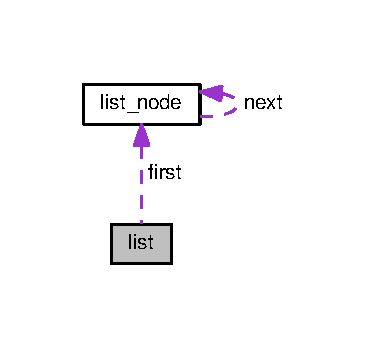
\includegraphics[width=176pt]{structlist__coll__graph}
\end{center}
\end{figure}
\subsection*{Data Fields}
\begin{DoxyCompactItemize}
\item 
size\+\_\+t \textbf{ length}
\item 
struct \textbf{ list\+\_\+node} $\ast$ \textbf{ first}
\end{DoxyCompactItemize}


\subsection{Detailed Description}
Head of a singly-\/linked list. 

\subsection{Field Documentation}
\mbox{\label{structlist_a15417ebe69a6b33324e8286dde558146}} 
\index{list@{list}!first@{first}}
\index{first@{first}!list@{list}}
\subsubsection{first}
{\footnotesize\ttfamily struct \textbf{ list\+\_\+node}$\ast$ first}

\mbox{\label{structlist_ae809d5359ac030c60a30a8f0b2294b82}} 
\index{list@{list}!length@{length}}
\index{length@{length}!list@{list}}
\subsubsection{length}
{\footnotesize\ttfamily size\+\_\+t length}



The documentation for this struct was generated from the following file\+:\begin{DoxyCompactItemize}
\item 
src/utils/\textbf{ list.\+h}\end{DoxyCompactItemize}

\section{list\+\_\+node Struct Reference}
\label{structlist__node}\index{list\+\_\+node@{list\+\_\+node}}


{\ttfamily \#include $<$list.\+h$>$}



Collaboration diagram for list\+\_\+node\+:
\nopagebreak
\begin{figure}[H]
\begin{center}
\leavevmode
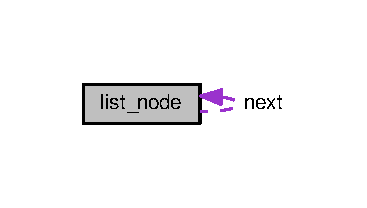
\includegraphics[width=176pt]{structlist__node__coll__graph}
\end{center}
\end{figure}
\subsection*{Data Fields}
\begin{DoxyCompactItemize}
\item 
struct \textbf{ list\+\_\+node} $\ast$ \textbf{ next}
\end{DoxyCompactItemize}


\subsection{Detailed Description}
A node of a singly-\/linked list. 

\subsection{Field Documentation}
\mbox{\label{structlist__node_a233bfe7cf29d581dfb42116900d0739f}} 
\index{list\+\_\+node@{list\+\_\+node}!next@{next}}
\index{next@{next}!list\+\_\+node@{list\+\_\+node}}
\subsubsection{next}
{\footnotesize\ttfamily struct \textbf{ list\+\_\+node}$\ast$ next}



The documentation for this struct was generated from the following file\+:\begin{DoxyCompactItemize}
\item 
src/utils/\textbf{ list.\+h}\end{DoxyCompactItemize}

\section{matrix Struct Reference}
\label{structmatrix}\index{matrix@{matrix}}


{\ttfamily \#include $<$matrix.\+h$>$}

\subsection*{Data Fields}
\begin{DoxyCompactItemize}
\item 
size\+\_\+t \textbf{ rows}
\item 
size\+\_\+t \textbf{ cols}
\item 
double $\ast$ \textbf{ data}
\end{DoxyCompactItemize}


\subsection{Detailed Description}
Matrix structure 

\subsection{Field Documentation}
\mbox{\label{structmatrix_a8bc05371b3a4013263f68932ba1b6452}} 
\index{matrix@{matrix}!cols@{cols}}
\index{cols@{cols}!matrix@{matrix}}
\subsubsection{cols}
{\footnotesize\ttfamily size\+\_\+t cols}

Columns \mbox{\label{structmatrix_a23436a7a2b44939627b59df11be7ad75}} 
\index{matrix@{matrix}!data@{data}}
\index{data@{data}!matrix@{matrix}}
\subsubsection{data}
{\footnotesize\ttfamily double$\ast$ data}

Values \mbox{\label{structmatrix_ad161320eba27a8b966baac47bee35c46}} 
\index{matrix@{matrix}!rows@{rows}}
\index{rows@{rows}!matrix@{matrix}}
\subsubsection{rows}
{\footnotesize\ttfamily size\+\_\+t rows}

Rows 

The documentation for this struct was generated from the following file\+:\begin{DoxyCompactItemize}
\item 
src/utils/\textbf{ matrix.\+h}\end{DoxyCompactItemize}

\chapter{File Documentation}
\section{src/t\+A\+Itris.c File Reference}
\label{tAItris_8c}\index{src/t\+A\+Itris.\+c@{src/t\+A\+Itris.\+c}}


Main file.  


{\ttfamily \#include \char`\"{}utils/random.\+h\char`\"{}}\newline
{\ttfamily \#include \char`\"{}engine/piece/piece\+\_\+queue.\+h\char`\"{}}\newline
{\ttfamily \#include \char`\"{}engine/state.\+h\char`\"{}}\newline
{\ttfamily \#include \char`\"{}debug/engine/debug\+\_\+state.\+h\char`\"{}}\newline
Include dependency graph for t\+A\+Itris.\+c\+:
\nopagebreak
\begin{figure}[H]
\begin{center}
\leavevmode
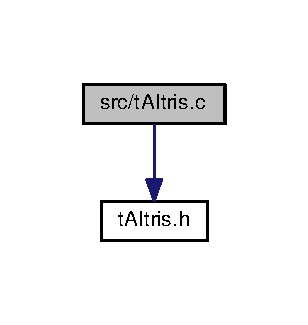
\includegraphics[width=350pt]{tAItris_8c__incl}
\end{center}
\end{figure}
\subsection*{Functions}
\begin{DoxyCompactItemize}
\item 
int \textbf{ main} ()
\end{DoxyCompactItemize}


\subsection{Detailed Description}
Main file. 

\begin{DoxyAuthor}{Author}
S4\+Master\+Race 
\end{DoxyAuthor}
\begin{DoxyVersion}{Version}
2.\+0 
\end{DoxyVersion}


\subsection{Function Documentation}
\mbox{\label{tAItris_8c_ae66f6b31b5ad750f1fe042a706a4e3d4}} 
\index{t\+A\+Itris.\+c@{t\+A\+Itris.\+c}!main@{main}}
\index{main@{main}!t\+A\+Itris.\+c@{t\+A\+Itris.\+c}}
\subsubsection{main()}
{\footnotesize\ttfamily int main (\begin{DoxyParamCaption}{ }\end{DoxyParamCaption})}


\section{src/t\+A\+Itris.h File Reference}
\label{tAItris_8h}\index{src/t\+A\+Itris.\+h@{src/t\+A\+Itris.\+h}}
This graph shows which files directly or indirectly include this file\+:
\nopagebreak
\begin{figure}[H]
\begin{center}
\leavevmode
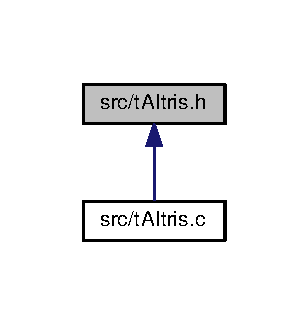
\includegraphics[width=148pt]{tAItris_8h__dep__incl}
\end{center}
\end{figure}

\section{src/utils/list.c File Reference}
\label{list_8c}\index{src/utils/list.\+c@{src/utils/list.\+c}}
{\ttfamily \#include \char`\"{}list.\+h\char`\"{}}\newline
Include dependency graph for list.\+c\+:
\nopagebreak
\begin{figure}[H]
\begin{center}
\leavevmode
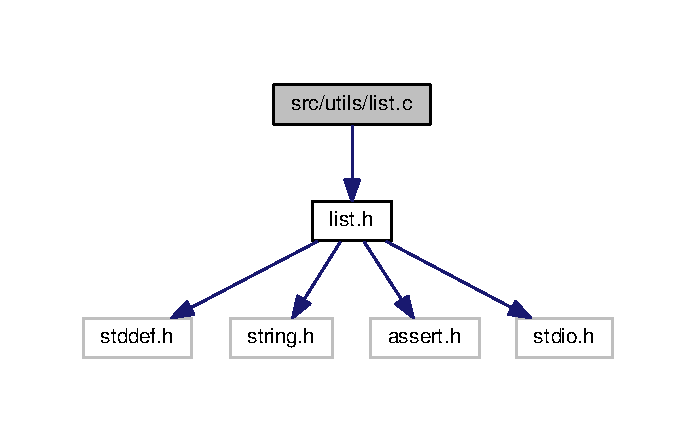
\includegraphics[width=334pt]{list_8c__incl}
\end{center}
\end{figure}
\subsection*{Functions}
\begin{DoxyCompactItemize}
\item 
void \textbf{ list\+\_\+init} (struct \textbf{ list} $\ast$\textbf{ list})
\item 
size\+\_\+t \textbf{ list\+\_\+length} (const struct \textbf{ list} $\ast$\textbf{ list})
\item 
struct \textbf{ list\+\_\+node} $\ast$ \textbf{ list\+\_\+first} (const struct \textbf{ list} $\ast$\textbf{ list})
\item 
struct \textbf{ list\+\_\+node} $\ast$ \textbf{ list\+\_\+last} (const struct \textbf{ list} $\ast$\textbf{ list})
\item 
struct \textbf{ list\+\_\+node} $\ast$ \textbf{ list\+\_\+next} (const struct \textbf{ list\+\_\+node} $\ast$node)
\item 
struct \textbf{ list\+\_\+node} $\ast$ \textbf{ list\+\_\+advance} (struct \textbf{ list\+\_\+node} $\ast$node, size\+\_\+t distance)
\item 
struct \textbf{ list\+\_\+node} $\ast$ \textbf{ list\+\_\+at} (const struct \textbf{ list} $\ast$\textbf{ list}, size\+\_\+t pos)
\item 
void \textbf{ list\+\_\+reverse} (struct \textbf{ list} $\ast$\textbf{ list})
\item 
void \textbf{ list\+\_\+swap} (struct \textbf{ list} $\ast$l1, struct \textbf{ list} $\ast$l2)
\item 
void \textbf{ list\+\_\+split\+\_\+at} (struct \textbf{ list} $\ast$\textbf{ list}, size\+\_\+t pos, struct \textbf{ list} $\ast$right)
\item 
void \textbf{ list\+\_\+concat} (struct \textbf{ list} $\ast$l1, struct \textbf{ list} $\ast$l2)
\item 
void \textbf{ list\+\_\+sort} (struct \textbf{ list} $\ast$\textbf{ list}, int($\ast$cmp)(struct \textbf{ list\+\_\+node} $\ast$, struct \textbf{ list\+\_\+node} $\ast$))
\item 
int \textbf{ list\+\_\+is\+\_\+empty} (const struct \textbf{ list} $\ast$\textbf{ list})
\item 
void \textbf{ list\+\_\+add} (struct \textbf{ list} $\ast$\textbf{ list}, struct \textbf{ list\+\_\+node} $\ast$node)
\item 
void \textbf{ list\+\_\+append} (struct \textbf{ list} $\ast$\textbf{ list}, struct \textbf{ list\+\_\+node} $\ast$node)
\item 
void \textbf{ list\+\_\+insert\+\_\+after} (struct \textbf{ list} $\ast$\textbf{ list}, struct \textbf{ list\+\_\+node} $\ast$curr, struct \textbf{ list\+\_\+node} $\ast$node)
\item 
void \textbf{ list\+\_\+insert\+\_\+at} (struct \textbf{ list} $\ast$\textbf{ list}, struct \textbf{ list\+\_\+node} $\ast$node, size\+\_\+t pos)
\item 
void \textbf{ list\+\_\+del} (struct \textbf{ list} $\ast$\textbf{ list})
\item 
void \textbf{ list\+\_\+del\+\_\+after} (struct \textbf{ list} $\ast$\textbf{ list}, struct \textbf{ list\+\_\+node} $\ast$node)
\item 
void \textbf{ list\+\_\+del\+\_\+at} (struct \textbf{ list} $\ast$\textbf{ list}, size\+\_\+t pos)
\item 
void \textbf{ list\+\_\+print} (struct \textbf{ list} $\ast$\textbf{ list})
\end{DoxyCompactItemize}


\subsection{Function Documentation}
\mbox{\label{list_8c_a9a78b4aa6e818c4b9e3da16cf3d1e9cf}} 
\index{list.\+c@{list.\+c}!list\+\_\+add@{list\+\_\+add}}
\index{list\+\_\+add@{list\+\_\+add}!list.\+c@{list.\+c}}
\subsubsection{list\+\_\+add()}
{\footnotesize\ttfamily void list\+\_\+add (\begin{DoxyParamCaption}\item[{struct \textbf{ list} $\ast$}]{list,  }\item[{struct \textbf{ list\+\_\+node} $\ast$}]{node }\end{DoxyParamCaption})\hspace{0.3cm}{\ttfamily [inline]}}

Adds {\ttfamily node} in the front of {\ttfamily list}


\begin{DoxyParams}{Parameters}
{\em list} & a list. \\
\hline
{\em node} & the new node.\\
\hline
\end{DoxyParams}
\begin{DoxyPrecond}{Precondition}
{\ttfamily list} must be not N\+U\+LL. 

{\ttfamily node} must be not N\+U\+LL.
\end{DoxyPrecond}
\begin{DoxyPostcond}{Postcondition}
List size increases by 1.
\end{DoxyPostcond}
\begin{DoxyRemark}{Remarks}
Complexity\+: O(1) 
\end{DoxyRemark}
\mbox{\label{list_8c_a3e71507d9a07668a357907d4515336de}} 
\index{list.\+c@{list.\+c}!list\+\_\+advance@{list\+\_\+advance}}
\index{list\+\_\+advance@{list\+\_\+advance}!list.\+c@{list.\+c}}
\subsubsection{list\+\_\+advance()}
{\footnotesize\ttfamily struct \textbf{ list\+\_\+node}$\ast$ list\+\_\+advance (\begin{DoxyParamCaption}\item[{struct \textbf{ list\+\_\+node} $\ast$}]{node,  }\item[{size\+\_\+t}]{distance }\end{DoxyParamCaption})}

Returns the nth-\/node after the current one.


\begin{DoxyParams}{Parameters}
{\em node} & a node. \\
\hline
{\em distance} & distance to move on. \\
\hline
\end{DoxyParams}
\begin{DoxyReturn}{Returns}
the nth-\/node after {\ttfamily node}.
\end{DoxyReturn}
\begin{DoxyPrecond}{Precondition}
{\ttfamily node} must be not N\+U\+LL.
\end{DoxyPrecond}
\begin{DoxyRemark}{Remarks}
Complexity\+: O(n) 
\end{DoxyRemark}
\mbox{\label{list_8c_a40638777b5f341c88e8b09acf75fb8c9}} 
\index{list.\+c@{list.\+c}!list\+\_\+append@{list\+\_\+append}}
\index{list\+\_\+append@{list\+\_\+append}!list.\+c@{list.\+c}}
\subsubsection{list\+\_\+append()}
{\footnotesize\ttfamily void list\+\_\+append (\begin{DoxyParamCaption}\item[{struct \textbf{ list} $\ast$}]{list,  }\item[{struct \textbf{ list\+\_\+node} $\ast$}]{node }\end{DoxyParamCaption})\hspace{0.3cm}{\ttfamily [inline]}}

Adds {\ttfamily node} at the end of {\ttfamily list}.


\begin{DoxyParams}{Parameters}
{\em list} & a list. \\
\hline
{\em node} & the new node.\\
\hline
\end{DoxyParams}
\begin{DoxyPrecond}{Precondition}
{\ttfamily list} must be not N\+U\+LL. 

{\ttfamily node} must be not N\+U\+LL.
\end{DoxyPrecond}
\begin{DoxyPostcond}{Postcondition}
List size increases by 1.
\end{DoxyPostcond}
\begin{DoxyRemark}{Remarks}
Complexity\+: O(n) 
\end{DoxyRemark}
\mbox{\label{list_8c_abcf02e7a58093a7b70a84be889da4aad}} 
\index{list.\+c@{list.\+c}!list\+\_\+at@{list\+\_\+at}}
\index{list\+\_\+at@{list\+\_\+at}!list.\+c@{list.\+c}}
\subsubsection{list\+\_\+at()}
{\footnotesize\ttfamily struct \textbf{ list\+\_\+node}$\ast$ list\+\_\+at (\begin{DoxyParamCaption}\item[{const struct \textbf{ list} $\ast$}]{list,  }\item[{size\+\_\+t}]{pos }\end{DoxyParamCaption})}

Returns node at the position {\ttfamily pos}.


\begin{DoxyParams}{Parameters}
{\em list} & a list. \\
\hline
{\em pos} & position (0-\/based) of the node. \\
\hline
\end{DoxyParams}
\begin{DoxyReturn}{Returns}
the node at the position {\ttfamily pos}.
\end{DoxyReturn}
\begin{DoxyPrecond}{Precondition}
{\ttfamily list} must be not N\+U\+LL. 

{\ttfamily list} must be not empty. 

{\ttfamily pos} must be in [0; list\+\_\+length(list)[.
\end{DoxyPrecond}
\begin{DoxyRemark}{Remarks}
Complexity\+: O(\+N) 
\end{DoxyRemark}
\mbox{\label{list_8c_af71fffc666f138957b1e015fdae5fe1f}} 
\index{list.\+c@{list.\+c}!list\+\_\+concat@{list\+\_\+concat}}
\index{list\+\_\+concat@{list\+\_\+concat}!list.\+c@{list.\+c}}
\subsubsection{list\+\_\+concat()}
{\footnotesize\ttfamily void list\+\_\+concat (\begin{DoxyParamCaption}\item[{struct \textbf{ list} $\ast$}]{l1,  }\item[{struct \textbf{ list} $\ast$}]{l2 }\end{DoxyParamCaption})\hspace{0.3cm}{\ttfamily [inline]}}

Concatenates two lists.


\begin{DoxyParams}{Parameters}
{\em l1} & list 1. \\
\hline
{\em l2} & list 2.\\
\hline
\end{DoxyParams}
\begin{DoxyPrecond}{Precondition}
{\ttfamily l1} must be not N\+U\+LL. 

{\ttfamily l2} must be not N\+U\+LL. 

{\ttfamily l1} must be different of {\ttfamily l2}.
\end{DoxyPrecond}
\begin{DoxyPostcond}{Postcondition}
{\ttfamily l2} is reset to an empty list.
\end{DoxyPostcond}
\begin{DoxyRemark}{Remarks}
Complexity\+: O(\+N) 
\end{DoxyRemark}
\mbox{\label{list_8c_a4ee9116bc5b8f1b5da93f415d8529d58}} 
\index{list.\+c@{list.\+c}!list\+\_\+del@{list\+\_\+del}}
\index{list\+\_\+del@{list\+\_\+del}!list.\+c@{list.\+c}}
\subsubsection{list\+\_\+del()}
{\footnotesize\ttfamily void list\+\_\+del (\begin{DoxyParamCaption}\item[{struct \textbf{ list} $\ast$}]{list }\end{DoxyParamCaption})\hspace{0.3cm}{\ttfamily [inline]}}

Deletes the first node.


\begin{DoxyParams}{Parameters}
{\em list} & a list.\\
\hline
\end{DoxyParams}
\begin{DoxyPrecond}{Precondition}
{\ttfamily list} must be not N\+U\+LL. 

{\ttfamily list} must be not empty.
\end{DoxyPrecond}
\begin{DoxyPostcond}{Postcondition}
List size decreases by 1.
\end{DoxyPostcond}
\begin{DoxyRemark}{Remarks}
Complexity\+: O(1) 
\end{DoxyRemark}
\mbox{\label{list_8c_ad301311c004c0b56091e2e89e5a1f5e8}} 
\index{list.\+c@{list.\+c}!list\+\_\+del\+\_\+after@{list\+\_\+del\+\_\+after}}
\index{list\+\_\+del\+\_\+after@{list\+\_\+del\+\_\+after}!list.\+c@{list.\+c}}
\subsubsection{list\+\_\+del\+\_\+after()}
{\footnotesize\ttfamily void list\+\_\+del\+\_\+after (\begin{DoxyParamCaption}\item[{struct \textbf{ list} $\ast$}]{list,  }\item[{struct \textbf{ list\+\_\+node} $\ast$}]{node }\end{DoxyParamCaption})\hspace{0.3cm}{\ttfamily [inline]}}

Deletes the node at after the node {\ttfamily curr}.


\begin{DoxyParams}{Parameters}
{\em list} & a list. \\
\hline
{\em node} & a node of {\ttfamily list}.\\
\hline
\end{DoxyParams}
\begin{DoxyPrecond}{Precondition}
{\ttfamily list} must be not N\+U\+LL. 

{\ttfamily node} must be not N\+U\+LL. 

{\ttfamily list} must be not empty. 

{\ttfamily node} must a node of {\ttfamily list}.
\end{DoxyPrecond}
\begin{DoxyPostcond}{Postcondition}
List size decreases by 1.
\end{DoxyPostcond}
\begin{DoxyRemark}{Remarks}
Complexity\+: O(1) 
\end{DoxyRemark}
\mbox{\label{list_8c_a1b32056f04fe6cce76bc8774b462598f}} 
\index{list.\+c@{list.\+c}!list\+\_\+del\+\_\+at@{list\+\_\+del\+\_\+at}}
\index{list\+\_\+del\+\_\+at@{list\+\_\+del\+\_\+at}!list.\+c@{list.\+c}}
\subsubsection{list\+\_\+del\+\_\+at()}
{\footnotesize\ttfamily void list\+\_\+del\+\_\+at (\begin{DoxyParamCaption}\item[{struct \textbf{ list} $\ast$}]{list,  }\item[{size\+\_\+t}]{pos }\end{DoxyParamCaption})\hspace{0.3cm}{\ttfamily [inline]}}

Deletes the node at the position {\ttfamily pos}.


\begin{DoxyParams}{Parameters}
{\em list} & a list. \\
\hline
{\em pos} & index (0-\/based) of the node to delete.\\
\hline
\end{DoxyParams}
\begin{DoxyPrecond}{Precondition}
{\ttfamily list} must be not N\+U\+LL. 

{\ttfamily list} must be not empty. 

{\ttfamily pos} must be in [0; list\+\_\+length(list)[.
\end{DoxyPrecond}
\begin{DoxyPostcond}{Postcondition}
List size decreases by 1.
\end{DoxyPostcond}
\begin{DoxyRemark}{Remarks}
Complexity\+: O(n) 
\end{DoxyRemark}
\mbox{\label{list_8c_ab31246f096207d08b4756bd2c209fa2b}} 
\index{list.\+c@{list.\+c}!list\+\_\+first@{list\+\_\+first}}
\index{list\+\_\+first@{list\+\_\+first}!list.\+c@{list.\+c}}
\subsubsection{list\+\_\+first()}
{\footnotesize\ttfamily struct \textbf{ list\+\_\+node}$\ast$ list\+\_\+first (\begin{DoxyParamCaption}\item[{const struct \textbf{ list} $\ast$}]{list }\end{DoxyParamCaption})}

Returns the first node.


\begin{DoxyParams}{Parameters}
{\em list} & a list. \\
\hline
\end{DoxyParams}
\begin{DoxyReturn}{Returns}
the first node.
\end{DoxyReturn}
\begin{DoxyPrecond}{Precondition}
{\ttfamily list} must be not N\+U\+LL. 

{\ttfamily list} must be not empty.
\end{DoxyPrecond}
\begin{DoxyRemark}{Remarks}
Complexity\+: O(1) 
\end{DoxyRemark}
\mbox{\label{list_8c_a8aa862d10f52f7b0348fce990c7c12db}} 
\index{list.\+c@{list.\+c}!list\+\_\+init@{list\+\_\+init}}
\index{list\+\_\+init@{list\+\_\+init}!list.\+c@{list.\+c}}
\subsubsection{list\+\_\+init()}
{\footnotesize\ttfamily void list\+\_\+init (\begin{DoxyParamCaption}\item[{struct \textbf{ list} $\ast$}]{list }\end{DoxyParamCaption})\hspace{0.3cm}{\ttfamily [inline]}}

Initializes the list.


\begin{DoxyParams}{Parameters}
{\em list} & a list.\\
\hline
\end{DoxyParams}
\begin{DoxyPrecond}{Precondition}
{\ttfamily list} must be not N\+U\+LL.
\end{DoxyPrecond}
\begin{DoxyPostcond}{Postcondition}
{\ttfamily list} is empty. 

{\ttfamily list} has a size of 0.
\end{DoxyPostcond}
\begin{DoxyRemark}{Remarks}
Complexity\+: O(1) 
\end{DoxyRemark}
\mbox{\label{list_8c_aac5b9656592776dd99c192c7c8f2b18f}} 
\index{list.\+c@{list.\+c}!list\+\_\+insert\+\_\+after@{list\+\_\+insert\+\_\+after}}
\index{list\+\_\+insert\+\_\+after@{list\+\_\+insert\+\_\+after}!list.\+c@{list.\+c}}
\subsubsection{list\+\_\+insert\+\_\+after()}
{\footnotesize\ttfamily void list\+\_\+insert\+\_\+after (\begin{DoxyParamCaption}\item[{struct \textbf{ list} $\ast$}]{list,  }\item[{struct \textbf{ list\+\_\+node} $\ast$}]{curr,  }\item[{struct \textbf{ list\+\_\+node} $\ast$}]{node }\end{DoxyParamCaption})\hspace{0.3cm}{\ttfamily [inline]}}

Inserts {\ttfamily node} at after the node {\ttfamily curr}.


\begin{DoxyParams}{Parameters}
{\em list} & a list. \\
\hline
{\em curr} & a node of {\ttfamily list}. \\
\hline
{\em node} & new node.\\
\hline
\end{DoxyParams}
\begin{DoxyPrecond}{Precondition}
{\ttfamily list} must be not N\+U\+LL. 

{\ttfamily curr} must be not N\+U\+LL. 

{\ttfamily curr} must a node of {\ttfamily list}. 

{\ttfamily node} must be not N\+U\+LL.
\end{DoxyPrecond}
\begin{DoxyPostcond}{Postcondition}
List size increases by 1.
\end{DoxyPostcond}
\begin{DoxyRemark}{Remarks}
Complexity\+: O(1) 
\end{DoxyRemark}
\mbox{\label{list_8c_a7f9a331cc4eab17800dc8fac961b50c9}} 
\index{list.\+c@{list.\+c}!list\+\_\+insert\+\_\+at@{list\+\_\+insert\+\_\+at}}
\index{list\+\_\+insert\+\_\+at@{list\+\_\+insert\+\_\+at}!list.\+c@{list.\+c}}
\subsubsection{list\+\_\+insert\+\_\+at()}
{\footnotesize\ttfamily void list\+\_\+insert\+\_\+at (\begin{DoxyParamCaption}\item[{struct \textbf{ list} $\ast$}]{list,  }\item[{struct \textbf{ list\+\_\+node} $\ast$}]{node,  }\item[{size\+\_\+t}]{pos }\end{DoxyParamCaption})\hspace{0.3cm}{\ttfamily [inline]}}

Inserts {\ttfamily node} at the position {\ttfamily pos} in {\ttfamily list}.


\begin{DoxyParams}{Parameters}
{\em list} & a list. \\
\hline
{\em node} & new node. \\
\hline
{\em pos} & position (0-\/based) where to insert the new node.\\
\hline
\end{DoxyParams}
\begin{DoxyPrecond}{Precondition}
{\ttfamily list} must be not N\+U\+LL. 

{\ttfamily node} must be not N\+U\+LL. 

{\ttfamily pos} must be in [0; list\+\_\+length(list)].
\end{DoxyPrecond}
\begin{DoxyPostcond}{Postcondition}
List size increases by 1.
\end{DoxyPostcond}
\begin{DoxyRemark}{Remarks}
Complexity\+: O(n) 
\end{DoxyRemark}
\mbox{\label{list_8c_aa1c6d252fce51c8ebed845bf8fbcfdb7}} 
\index{list.\+c@{list.\+c}!list\+\_\+is\+\_\+empty@{list\+\_\+is\+\_\+empty}}
\index{list\+\_\+is\+\_\+empty@{list\+\_\+is\+\_\+empty}!list.\+c@{list.\+c}}
\subsubsection{list\+\_\+is\+\_\+empty()}
{\footnotesize\ttfamily int list\+\_\+is\+\_\+empty (\begin{DoxyParamCaption}\item[{const struct \textbf{ list} $\ast$}]{list }\end{DoxyParamCaption})\hspace{0.3cm}{\ttfamily [inline]}}

Tests if a list is empty.


\begin{DoxyParams}{Parameters}
{\em list} & a list. \\
\hline
\end{DoxyParams}
\begin{DoxyReturn}{Returns}
1 if the list is empty, otherwise 0.
\end{DoxyReturn}
\begin{DoxyPrecond}{Precondition}
{\ttfamily list} must be not N\+U\+LL.
\end{DoxyPrecond}
\begin{DoxyRemark}{Remarks}
Complexity\+: O(1) 
\end{DoxyRemark}
\mbox{\label{list_8c_a5a3f95e5d8edeb9ff16d4ce0d0ceac95}} 
\index{list.\+c@{list.\+c}!list\+\_\+last@{list\+\_\+last}}
\index{list\+\_\+last@{list\+\_\+last}!list.\+c@{list.\+c}}
\subsubsection{list\+\_\+last()}
{\footnotesize\ttfamily struct \textbf{ list\+\_\+node}$\ast$ list\+\_\+last (\begin{DoxyParamCaption}\item[{const struct \textbf{ list} $\ast$}]{list }\end{DoxyParamCaption})}

Returns the last node.


\begin{DoxyParams}{Parameters}
{\em list} & a list. \\
\hline
\end{DoxyParams}
\begin{DoxyReturn}{Returns}
the last node.
\end{DoxyReturn}
\begin{DoxyPrecond}{Precondition}
{\ttfamily list} must be not N\+U\+LL.
\end{DoxyPrecond}
\begin{DoxyRemark}{Remarks}
Complexity\+: O(\+N) 
\end{DoxyRemark}
\mbox{\label{list_8c_a5ded68cde03f48a724bb04326dc5cc87}} 
\index{list.\+c@{list.\+c}!list\+\_\+length@{list\+\_\+length}}
\index{list\+\_\+length@{list\+\_\+length}!list.\+c@{list.\+c}}
\subsubsection{list\+\_\+length()}
{\footnotesize\ttfamily size\+\_\+t list\+\_\+length (\begin{DoxyParamCaption}\item[{const struct \textbf{ list} $\ast$}]{list }\end{DoxyParamCaption})\hspace{0.3cm}{\ttfamily [inline]}}

Returns the size of the list.


\begin{DoxyParams}{Parameters}
{\em list} & a list. \\
\hline
\end{DoxyParams}
\begin{DoxyReturn}{Returns}
the length of the list.
\end{DoxyReturn}
\begin{DoxyPrecond}{Precondition}
{\ttfamily list} must be not N\+U\+LL.
\end{DoxyPrecond}
\begin{DoxyRemark}{Remarks}
Complexity\+: O(1) 
\end{DoxyRemark}
\mbox{\label{list_8c_aa2253e2e4f2da4eb7a3b17759369dcd7}} 
\index{list.\+c@{list.\+c}!list\+\_\+next@{list\+\_\+next}}
\index{list\+\_\+next@{list\+\_\+next}!list.\+c@{list.\+c}}
\subsubsection{list\+\_\+next()}
{\footnotesize\ttfamily struct \textbf{ list\+\_\+node}$\ast$ list\+\_\+next (\begin{DoxyParamCaption}\item[{const struct \textbf{ list\+\_\+node} $\ast$}]{node }\end{DoxyParamCaption})}

Returns the next node.


\begin{DoxyParams}{Parameters}
{\em node} & a node. \\
\hline
\end{DoxyParams}
\begin{DoxyReturn}{Returns}
the next node.
\end{DoxyReturn}
\begin{DoxyPrecond}{Precondition}
{\ttfamily node} must be not N\+U\+LL.
\end{DoxyPrecond}
\begin{DoxyRemark}{Remarks}
Complexity\+: O(1) 
\end{DoxyRemark}
\mbox{\label{list_8c_a16d4d495efa468873a1afafb7a353e38}} 
\index{list.\+c@{list.\+c}!list\+\_\+print@{list\+\_\+print}}
\index{list\+\_\+print@{list\+\_\+print}!list.\+c@{list.\+c}}
\subsubsection{list\+\_\+print()}
{\footnotesize\ttfamily void list\+\_\+print (\begin{DoxyParamCaption}\item[{struct \textbf{ list} $\ast$}]{list }\end{DoxyParamCaption})}

Print the list


\begin{DoxyParams}{Parameters}
{\em list} & a list \\
\hline
\end{DoxyParams}
\mbox{\label{list_8c_ac2bed4543182c599319388b26e10811f}} 
\index{list.\+c@{list.\+c}!list\+\_\+reverse@{list\+\_\+reverse}}
\index{list\+\_\+reverse@{list\+\_\+reverse}!list.\+c@{list.\+c}}
\subsubsection{list\+\_\+reverse()}
{\footnotesize\ttfamily void list\+\_\+reverse (\begin{DoxyParamCaption}\item[{struct \textbf{ list} $\ast$}]{list }\end{DoxyParamCaption})\hspace{0.3cm}{\ttfamily [inline]}}

Reverses the order of the elements in the list.


\begin{DoxyParams}{Parameters}
{\em list} & a list.\\
\hline
\end{DoxyParams}
\begin{DoxyPrecond}{Precondition}
{\ttfamily list} must be not N\+U\+LL.
\end{DoxyPrecond}
\begin{DoxyRemark}{Remarks}
Complexity\+: O(\+N) 
\end{DoxyRemark}
\mbox{\label{list_8c_aafd30da5da0e55fa5510328f579e7830}} 
\index{list.\+c@{list.\+c}!list\+\_\+sort@{list\+\_\+sort}}
\index{list\+\_\+sort@{list\+\_\+sort}!list.\+c@{list.\+c}}
\subsubsection{list\+\_\+sort()}
{\footnotesize\ttfamily void list\+\_\+sort (\begin{DoxyParamCaption}\item[{struct \textbf{ list} $\ast$}]{list,  }\item[{int($\ast$)(struct \textbf{ list\+\_\+node} $\ast$, struct \textbf{ list\+\_\+node} $\ast$)}]{cmp }\end{DoxyParamCaption})\hspace{0.3cm}{\ttfamily [inline]}}

Sort a list using a comparison function.

The contents of the list are sorted in ascending order according to a comparison function which is called with two arguments that point to the node being compared.

The comparison function must return an integer less than, equal to, or greater than zero if the first argument is considered to be respectively less than, equal to, or greater than the second.

If two members compare as equal, their order in the sorted list is preserved.


\begin{DoxyParams}{Parameters}
{\em list} & list to sort. \\
\hline
{\em cmp} & comparison function to use.\\
\hline
\end{DoxyParams}
\begin{DoxyPrecond}{Precondition}
{\ttfamily list} must be not N\+U\+LL. 

{\ttfamily cmp} must be not N\+U\+LL.
\end{DoxyPrecond}
\begin{DoxyRemark}{Remarks}
The sort is stable. 

Complexity\+: O(\+N log N) 

Space complexity\+: O(1) 
\end{DoxyRemark}
\mbox{\label{list_8c_ac55d3781f4c83cba6000c29161e3a419}} 
\index{list.\+c@{list.\+c}!list\+\_\+split\+\_\+at@{list\+\_\+split\+\_\+at}}
\index{list\+\_\+split\+\_\+at@{list\+\_\+split\+\_\+at}!list.\+c@{list.\+c}}
\subsubsection{list\+\_\+split\+\_\+at()}
{\footnotesize\ttfamily void list\+\_\+split\+\_\+at (\begin{DoxyParamCaption}\item[{struct \textbf{ list} $\ast$}]{list,  }\item[{size\+\_\+t}]{pos,  }\item[{struct \textbf{ list} $\ast$}]{right }\end{DoxyParamCaption})\hspace{0.3cm}{\ttfamily [inline]}}

Splits a list in two parts at the position {\ttfamily pos}.

After the split\+: \begin{DoxyItemize}
\item {\ttfamily list} contains nodes in [0, pos[ \item {\ttfamily right} contains nodes in [pos,length(list)[\end{DoxyItemize}
Examples\+: 
\begin{DoxyCode}
list = [1, 2, 3]
list_split_at(list, 0, right) => ([],[1,2,3])
list_split_at(list, 1, right) => ([1],[2,3])
list_split_at(list, 2, right) => ([1,2],[3])
list_split_at(list, 3, right) => ([1,2,3],[])
list = []
list_split_at(list, 0, right) => ([],[])
\end{DoxyCode}



\begin{DoxyParams}{Parameters}
{\em list} & list to split. \\
\hline
{\em pos} & position (0-\/based) where to split the list. \\
\hline
{\em right} & an empty list to receive the part after {\ttfamily pos}\\
\hline
\end{DoxyParams}
\begin{DoxyPrecond}{Precondition}
{\ttfamily list} must be not N\+U\+LL. 

{\ttfamily right} must be not N\+U\+LL. 

{\ttfamily right} must be empty. 

{\ttfamily list} must be different of {\ttfamily right}.
\end{DoxyPrecond}
\begin{DoxyRemark}{Remarks}
Complexity\+: O(\+N) 
\end{DoxyRemark}
\mbox{\label{list_8c_a41faf68fcdb7ac3c5d8a9168acd2a331}} 
\index{list.\+c@{list.\+c}!list\+\_\+swap@{list\+\_\+swap}}
\index{list\+\_\+swap@{list\+\_\+swap}!list.\+c@{list.\+c}}
\subsubsection{list\+\_\+swap()}
{\footnotesize\ttfamily void list\+\_\+swap (\begin{DoxyParamCaption}\item[{struct \textbf{ list} $\ast$}]{l1,  }\item[{struct \textbf{ list} $\ast$}]{l2 }\end{DoxyParamCaption})\hspace{0.3cm}{\ttfamily [inline]}}

Swaps two lists.


\begin{DoxyParams}{Parameters}
{\em l1} & list 1. \\
\hline
{\em l2} & list 2.\\
\hline
\end{DoxyParams}
\begin{DoxyPrecond}{Precondition}
{\ttfamily l1} must be not N\+U\+LL. 

{\ttfamily l2} must be not N\+U\+LL. 

{\ttfamily l1} must be different of {\ttfamily l2}.
\end{DoxyPrecond}
\begin{DoxyRemark}{Remarks}
Complexity\+: O(1) 
\end{DoxyRemark}

\section{src/utils/list.h File Reference}
\label{list_8h}\index{src/utils/list.\+h@{src/utils/list.\+h}}


Intrusive list implement.  


{\ttfamily \#include $<$stddef.\+h$>$}\newline
{\ttfamily \#include $<$string.\+h$>$}\newline
{\ttfamily \#include $<$assert.\+h$>$}\newline
{\ttfamily \#include $<$stdio.\+h$>$}\newline
Include dependency graph for list.\+h\+:\nopagebreak
\begin{figure}[H]
\begin{center}
\leavevmode
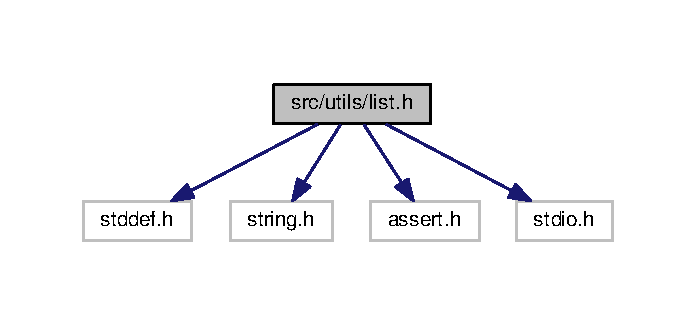
\includegraphics[width=334pt]{list_8h__incl}
\end{center}
\end{figure}
This graph shows which files directly or indirectly include this file\+:
\nopagebreak
\begin{figure}[H]
\begin{center}
\leavevmode
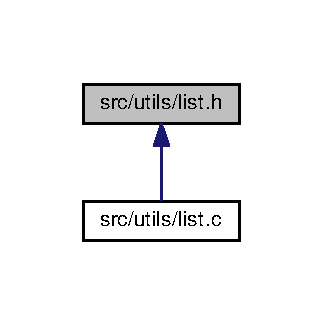
\includegraphics[width=155pt]{list_8h__dep__incl}
\end{center}
\end{figure}
\subsection*{Data Structures}
\begin{DoxyCompactItemize}
\item 
struct \textbf{ list}
\item 
struct \textbf{ list\+\_\+node}
\end{DoxyCompactItemize}
\subsection*{Macros}
\begin{DoxyCompactItemize}
\item 
\#define \textbf{ list\+\_\+elt}(node,  type,  fieldname)~((type$\ast$)((char$\ast$)(node) -\/ offsetof(type, fieldname)))
\item 
\#define \textbf{ list\+\_\+foreach}(\textbf{ list},  curr)~for (curr = \textbf{ list\+\_\+first}(\textbf{ list}); curr != N\+U\+LL; curr = \textbf{ list\+\_\+next}(curr))
\item 
\#define \textbf{ list\+\_\+foreach\+\_\+elt}(\textbf{ list},  curr,  type,  fieldname)
\item 
\#define \textbf{ list\+\_\+foreach\+\_\+safe}(\textbf{ list},  curr,  tmp)
\item 
\#define \textbf{ list\+\_\+foreach\+\_\+elt\+\_\+safe}(\textbf{ list},  curr,  tmp,  type,  fieldname)
\end{DoxyCompactItemize}
\subsection*{Functions}
\begin{DoxyCompactItemize}
\item 
void \textbf{ list\+\_\+init} (struct \textbf{ list} $\ast$\textbf{ list})
\item 
size\+\_\+t \textbf{ list\+\_\+length} (const struct \textbf{ list} $\ast$\textbf{ list})
\item 
struct \textbf{ list\+\_\+node} $\ast$ \textbf{ list\+\_\+first} (const struct \textbf{ list} $\ast$\textbf{ list})
\item 
struct \textbf{ list\+\_\+node} $\ast$ \textbf{ list\+\_\+last} (const struct \textbf{ list} $\ast$\textbf{ list})
\item 
struct \textbf{ list\+\_\+node} $\ast$ \textbf{ list\+\_\+next} (const struct \textbf{ list\+\_\+node} $\ast$node)
\item 
struct \textbf{ list\+\_\+node} $\ast$ \textbf{ list\+\_\+advance} (struct \textbf{ list\+\_\+node} $\ast$node, size\+\_\+t distance)
\item 
struct \textbf{ list\+\_\+node} $\ast$ \textbf{ list\+\_\+at} (const struct \textbf{ list} $\ast$\textbf{ list}, size\+\_\+t pos)
\item 
void \textbf{ list\+\_\+reverse} (struct \textbf{ list} $\ast$\textbf{ list})
\item 
void \textbf{ list\+\_\+swap} (struct \textbf{ list} $\ast$l1, struct \textbf{ list} $\ast$l2)
\item 
void \textbf{ list\+\_\+split\+\_\+at} (struct \textbf{ list} $\ast$\textbf{ list}, size\+\_\+t pos, struct \textbf{ list} $\ast$right)
\item 
void \textbf{ list\+\_\+concat} (struct \textbf{ list} $\ast$l1, struct \textbf{ list} $\ast$l2)
\item 
void \textbf{ list\+\_\+sort} (struct \textbf{ list} $\ast$\textbf{ list}, int($\ast$cmp)(struct \textbf{ list\+\_\+node} $\ast$, struct \textbf{ list\+\_\+node} $\ast$))
\item 
int \textbf{ list\+\_\+is\+\_\+empty} (const struct \textbf{ list} $\ast$\textbf{ list})
\item 
void \textbf{ list\+\_\+add} (struct \textbf{ list} $\ast$\textbf{ list}, struct \textbf{ list\+\_\+node} $\ast$node)
\item 
void \textbf{ list\+\_\+append} (struct \textbf{ list} $\ast$\textbf{ list}, struct \textbf{ list\+\_\+node} $\ast$node)
\item 
void \textbf{ list\+\_\+insert\+\_\+after} (struct \textbf{ list} $\ast$\textbf{ list}, struct \textbf{ list\+\_\+node} $\ast$curr, struct \textbf{ list\+\_\+node} $\ast$node)
\item 
void \textbf{ list\+\_\+insert\+\_\+at} (struct \textbf{ list} $\ast$\textbf{ list}, struct \textbf{ list\+\_\+node} $\ast$node, size\+\_\+t pos)
\item 
void \textbf{ list\+\_\+del} (struct \textbf{ list} $\ast$\textbf{ list})
\item 
void \textbf{ list\+\_\+del\+\_\+after} (struct \textbf{ list} $\ast$\textbf{ list}, struct \textbf{ list\+\_\+node} $\ast$node)
\item 
void \textbf{ list\+\_\+del\+\_\+at} (struct \textbf{ list} $\ast$\textbf{ list}, size\+\_\+t pos)
\item 
void \textbf{ list\+\_\+print} (const struct \textbf{ list} $\ast$\textbf{ list})
\end{DoxyCompactItemize}


\subsection{Detailed Description}
Intrusive list implement. 

\begin{DoxyAuthor}{Author}
S4\+Master\+Race 
\end{DoxyAuthor}
\begin{DoxyVersion}{Version}
1.\+0 
\end{DoxyVersion}


\subsection{Macro Definition Documentation}
\mbox{\label{list_8h_a12e153fb4ee7d1a550fa57a733629eac}} 
\index{list.\+h@{list.\+h}!list\+\_\+elt@{list\+\_\+elt}}
\index{list\+\_\+elt@{list\+\_\+elt}!list.\+h@{list.\+h}}
\subsubsection{list\+\_\+elt}
{\footnotesize\ttfamily \#define list\+\_\+elt(\begin{DoxyParamCaption}\item[{}]{node,  }\item[{}]{type,  }\item[{}]{fieldname }\end{DoxyParamCaption})~((type$\ast$)((char$\ast$)(node) -\/ offsetof(type, fieldname)))}

Returns a pointer to the structure which contains the node.


\begin{DoxyParams}{Parameters}
{\em node} & a list node (struct list\+\_\+node$\ast$). \\
\hline
{\em type} & type of the structure which contains the node. \\
\hline
{\em fieldname} & name of the node (field name) in the structure.\\
\hline
\end{DoxyParams}
\begin{DoxyPrecond}{Precondition}
{\ttfamily node} must be not N\+U\+LL.
\end{DoxyPrecond}
\begin{DoxyRemark}{Remarks}
Complexity\+: O(1) 
\end{DoxyRemark}
\mbox{\label{list_8h_a4cbdb4dde9bd442caf5bca5a01b891af}} 
\index{list.\+h@{list.\+h}!list\+\_\+foreach@{list\+\_\+foreach}}
\index{list\+\_\+foreach@{list\+\_\+foreach}!list.\+h@{list.\+h}}
\subsubsection{list\+\_\+foreach}
{\footnotesize\ttfamily \#define list\+\_\+foreach(\begin{DoxyParamCaption}\item[{}]{\textbf{ list},  }\item[{}]{curr }\end{DoxyParamCaption})~for (curr = \textbf{ list\+\_\+first}(\textbf{ list}); curr != N\+U\+LL; curr = \textbf{ list\+\_\+next}(curr))}

Iterates over list (nodes). 
\begin{DoxyParams}{Parameters}
{\em list} & a list (struct list$\ast$). \\
\hline
{\em curr} & a struct list\+\_\+node$\ast$ used to hold the current element.\\
\hline
\end{DoxyParams}
\begin{DoxyPrecond}{Precondition}
{\ttfamily list} must be not N\+U\+LL. 

{\ttfamily curr} must be not N\+U\+LL.
\end{DoxyPrecond}
\begin{DoxyRemark}{Remarks}
Complexity\+: O(\+N) 
\end{DoxyRemark}
\mbox{\label{list_8h_a007b1aa63bb2db9f0dc5e7947fb28ee9}} 
\index{list.\+h@{list.\+h}!list\+\_\+foreach\+\_\+elt@{list\+\_\+foreach\+\_\+elt}}
\index{list\+\_\+foreach\+\_\+elt@{list\+\_\+foreach\+\_\+elt}!list.\+h@{list.\+h}}
\subsubsection{list\+\_\+foreach\+\_\+elt}
{\footnotesize\ttfamily \#define list\+\_\+foreach\+\_\+elt(\begin{DoxyParamCaption}\item[{}]{\textbf{ list},  }\item[{}]{curr,  }\item[{}]{type,  }\item[{}]{fieldname }\end{DoxyParamCaption})}

{\bfseries Value\+:}
\begin{DoxyCode}
\textcolor{keywordflow}{for} (curr = list_elt(list_first(list), type, fieldname);       \(\backslash\)
         curr != NULL;                           \(\backslash\)
         curr = curr->fieldname.next == NULL ? NULL :           \(\backslash\)
         list\_elt(list_next(&(curr->fieldname)), type, fieldname))
\end{DoxyCode}
Iterates over list (elements) 
\begin{DoxyParams}{Parameters}
{\em list} & a list (struct list$\ast$). \\
\hline
{\em curr} & pointer (type$\ast$) used to hold the current element. \\
\hline
{\em type} & type of the structure which contains the node. \\
\hline
{\em fieldname} & name of the node (field name) in the structure.\\
\hline
\end{DoxyParams}
\begin{DoxyPrecond}{Precondition}
{\ttfamily list} must be not N\+U\+LL. 

{\ttfamily list} must be not empty. 

{\ttfamily curr} must be not N\+U\+LL.
\end{DoxyPrecond}
\begin{DoxyRemark}{Remarks}
Complexity\+: O(\+N) 
\end{DoxyRemark}
\mbox{\label{list_8h_a3ac4de28b3c9c2a36cf360390491afce}} 
\index{list.\+h@{list.\+h}!list\+\_\+foreach\+\_\+elt\+\_\+safe@{list\+\_\+foreach\+\_\+elt\+\_\+safe}}
\index{list\+\_\+foreach\+\_\+elt\+\_\+safe@{list\+\_\+foreach\+\_\+elt\+\_\+safe}!list.\+h@{list.\+h}}
\subsubsection{list\+\_\+foreach\+\_\+elt\+\_\+safe}
{\footnotesize\ttfamily \#define list\+\_\+foreach\+\_\+elt\+\_\+safe(\begin{DoxyParamCaption}\item[{}]{\textbf{ list},  }\item[{}]{curr,  }\item[{}]{tmp,  }\item[{}]{type,  }\item[{}]{fieldname }\end{DoxyParamCaption})}

{\bfseries Value\+:}
\begin{DoxyCode}
\textcolor{keywordflow}{for} (curr = list_elt(list_first(list), type, fieldname),      \(\backslash\)
         tmp  = list_next(&(curr->fieldname));              \(\backslash\)
         curr != NULL;                          \(\backslash\)
         curr = tmp == NULL ? NULL : list_elt(tmp, type, fieldname), \(\backslash\)
         tmp  = tmp == NULL ? NULL : list_next(tmp))          \(\backslash\)
\end{DoxyCode}
Iterates over list (elements), allows deletion of the current element. 
\begin{DoxyParams}{Parameters}
{\em list} & a list (struct list$\ast$). \\
\hline
{\em curr} & pointer (type$\ast$) used to hold the current element. \\
\hline
{\em tmp} & a struct list\+\_\+node$\ast$ used as temporary storage. \\
\hline
{\em type} & type of the structure which contains the node. \\
\hline
{\em fieldname} & name of the node (field name) in the structure.\\
\hline
\end{DoxyParams}
\begin{DoxyPrecond}{Precondition}
{\ttfamily list} must be not N\+U\+LL. 

{\ttfamily list} must be not empty. 

{\ttfamily curr} must be not N\+U\+LL.
\end{DoxyPrecond}
\begin{DoxyRemark}{Remarks}
Complexity\+: O(\+N) 
\end{DoxyRemark}
\mbox{\label{list_8h_a76d263fd3212139ab16fbd2d1bfd8a43}} 
\index{list.\+h@{list.\+h}!list\+\_\+foreach\+\_\+safe@{list\+\_\+foreach\+\_\+safe}}
\index{list\+\_\+foreach\+\_\+safe@{list\+\_\+foreach\+\_\+safe}!list.\+h@{list.\+h}}
\subsubsection{list\+\_\+foreach\+\_\+safe}
{\footnotesize\ttfamily \#define list\+\_\+foreach\+\_\+safe(\begin{DoxyParamCaption}\item[{}]{\textbf{ list},  }\item[{}]{curr,  }\item[{}]{tmp }\end{DoxyParamCaption})}

{\bfseries Value\+:}
\begin{DoxyCode}
\textcolor{keywordflow}{for} (curr = list_first(list), tmp = list_next(curr);    \(\backslash\)
         curr != NULL;                    \(\backslash\)
         curr = tmp, tmp = tmp == NULL ? NULL : list_next(tmp))
\end{DoxyCode}
Iterates over list (nodes), allows deletion of the current node. 
\begin{DoxyParams}{Parameters}
{\em list} & a list (struct list$\ast$). \\
\hline
{\em curr} & a struct list\+\_\+node$\ast$ used to hold the current element. \\
\hline
{\em tmp} & a struct list\+\_\+node$\ast$ used as temporary storage.\\
\hline
\end{DoxyParams}
\begin{DoxyPrecond}{Precondition}
{\ttfamily list} must be not N\+U\+LL. 

{\ttfamily curr} must be not N\+U\+LL. 

{\ttfamily tmp} must be not N\+U\+LL.
\end{DoxyPrecond}
\begin{DoxyRemark}{Remarks}
Complexity\+: O(\+N) 
\end{DoxyRemark}


\subsection{Function Documentation}
\mbox{\label{list_8h_a9a78b4aa6e818c4b9e3da16cf3d1e9cf}} 
\index{list.\+h@{list.\+h}!list\+\_\+add@{list\+\_\+add}}
\index{list\+\_\+add@{list\+\_\+add}!list.\+h@{list.\+h}}
\subsubsection{list\+\_\+add()}
{\footnotesize\ttfamily void list\+\_\+add (\begin{DoxyParamCaption}\item[{struct \textbf{ list} $\ast$}]{list,  }\item[{struct \textbf{ list\+\_\+node} $\ast$}]{node }\end{DoxyParamCaption})\hspace{0.3cm}{\ttfamily [inline]}}

Adds {\ttfamily node} in the front of {\ttfamily list}


\begin{DoxyParams}{Parameters}
{\em list} & a list. \\
\hline
{\em node} & the new node.\\
\hline
\end{DoxyParams}
\begin{DoxyPrecond}{Precondition}
{\ttfamily list} must be not N\+U\+LL. 

{\ttfamily node} must be not N\+U\+LL.
\end{DoxyPrecond}
\begin{DoxyPostcond}{Postcondition}
List size increases by 1.
\end{DoxyPostcond}
\begin{DoxyRemark}{Remarks}
Complexity\+: O(1) 
\end{DoxyRemark}
\mbox{\label{list_8h_a3e71507d9a07668a357907d4515336de}} 
\index{list.\+h@{list.\+h}!list\+\_\+advance@{list\+\_\+advance}}
\index{list\+\_\+advance@{list\+\_\+advance}!list.\+h@{list.\+h}}
\subsubsection{list\+\_\+advance()}
{\footnotesize\ttfamily struct \textbf{ list\+\_\+node}$\ast$ list\+\_\+advance (\begin{DoxyParamCaption}\item[{struct \textbf{ list\+\_\+node} $\ast$}]{node,  }\item[{size\+\_\+t}]{distance }\end{DoxyParamCaption})}

Returns the nth-\/node after the current one.


\begin{DoxyParams}{Parameters}
{\em node} & a node. \\
\hline
{\em distance} & distance to move on. \\
\hline
\end{DoxyParams}
\begin{DoxyReturn}{Returns}
the nth-\/node after {\ttfamily node}.
\end{DoxyReturn}
\begin{DoxyPrecond}{Precondition}
{\ttfamily node} must be not N\+U\+LL.
\end{DoxyPrecond}
\begin{DoxyRemark}{Remarks}
Complexity\+: O(n) 
\end{DoxyRemark}
\mbox{\label{list_8h_a40638777b5f341c88e8b09acf75fb8c9}} 
\index{list.\+h@{list.\+h}!list\+\_\+append@{list\+\_\+append}}
\index{list\+\_\+append@{list\+\_\+append}!list.\+h@{list.\+h}}
\subsubsection{list\+\_\+append()}
{\footnotesize\ttfamily void list\+\_\+append (\begin{DoxyParamCaption}\item[{struct \textbf{ list} $\ast$}]{list,  }\item[{struct \textbf{ list\+\_\+node} $\ast$}]{node }\end{DoxyParamCaption})\hspace{0.3cm}{\ttfamily [inline]}}

Adds {\ttfamily node} at the end of {\ttfamily list}.


\begin{DoxyParams}{Parameters}
{\em list} & a list. \\
\hline
{\em node} & the new node.\\
\hline
\end{DoxyParams}
\begin{DoxyPrecond}{Precondition}
{\ttfamily list} must be not N\+U\+LL. 

{\ttfamily node} must be not N\+U\+LL.
\end{DoxyPrecond}
\begin{DoxyPostcond}{Postcondition}
List size increases by 1.
\end{DoxyPostcond}
\begin{DoxyRemark}{Remarks}
Complexity\+: O(n) 
\end{DoxyRemark}
\mbox{\label{list_8h_abcf02e7a58093a7b70a84be889da4aad}} 
\index{list.\+h@{list.\+h}!list\+\_\+at@{list\+\_\+at}}
\index{list\+\_\+at@{list\+\_\+at}!list.\+h@{list.\+h}}
\subsubsection{list\+\_\+at()}
{\footnotesize\ttfamily struct \textbf{ list\+\_\+node}$\ast$ list\+\_\+at (\begin{DoxyParamCaption}\item[{const struct \textbf{ list} $\ast$}]{list,  }\item[{size\+\_\+t}]{pos }\end{DoxyParamCaption})}

Returns node at the position {\ttfamily pos}.


\begin{DoxyParams}{Parameters}
{\em list} & a list. \\
\hline
{\em pos} & position (0-\/based) of the node. \\
\hline
\end{DoxyParams}
\begin{DoxyReturn}{Returns}
the node at the position {\ttfamily pos}.
\end{DoxyReturn}
\begin{DoxyPrecond}{Precondition}
{\ttfamily list} must be not N\+U\+LL. 

{\ttfamily list} must be not empty. 

{\ttfamily pos} must be in [0; list\+\_\+length(list)[.
\end{DoxyPrecond}
\begin{DoxyRemark}{Remarks}
Complexity\+: O(\+N) 
\end{DoxyRemark}
\mbox{\label{list_8h_af71fffc666f138957b1e015fdae5fe1f}} 
\index{list.\+h@{list.\+h}!list\+\_\+concat@{list\+\_\+concat}}
\index{list\+\_\+concat@{list\+\_\+concat}!list.\+h@{list.\+h}}
\subsubsection{list\+\_\+concat()}
{\footnotesize\ttfamily void list\+\_\+concat (\begin{DoxyParamCaption}\item[{struct \textbf{ list} $\ast$}]{l1,  }\item[{struct \textbf{ list} $\ast$}]{l2 }\end{DoxyParamCaption})\hspace{0.3cm}{\ttfamily [inline]}}

Concatenates two lists.


\begin{DoxyParams}{Parameters}
{\em l1} & list 1. \\
\hline
{\em l2} & list 2.\\
\hline
\end{DoxyParams}
\begin{DoxyPrecond}{Precondition}
{\ttfamily l1} must be not N\+U\+LL. 

{\ttfamily l2} must be not N\+U\+LL. 

{\ttfamily l1} must be different of {\ttfamily l2}.
\end{DoxyPrecond}
\begin{DoxyPostcond}{Postcondition}
{\ttfamily l2} is reset to an empty list.
\end{DoxyPostcond}
\begin{DoxyRemark}{Remarks}
Complexity\+: O(\+N) 
\end{DoxyRemark}
\mbox{\label{list_8h_a4ee9116bc5b8f1b5da93f415d8529d58}} 
\index{list.\+h@{list.\+h}!list\+\_\+del@{list\+\_\+del}}
\index{list\+\_\+del@{list\+\_\+del}!list.\+h@{list.\+h}}
\subsubsection{list\+\_\+del()}
{\footnotesize\ttfamily void list\+\_\+del (\begin{DoxyParamCaption}\item[{struct \textbf{ list} $\ast$}]{list }\end{DoxyParamCaption})\hspace{0.3cm}{\ttfamily [inline]}}

Deletes the first node.


\begin{DoxyParams}{Parameters}
{\em list} & a list.\\
\hline
\end{DoxyParams}
\begin{DoxyPrecond}{Precondition}
{\ttfamily list} must be not N\+U\+LL. 

{\ttfamily list} must be not empty.
\end{DoxyPrecond}
\begin{DoxyPostcond}{Postcondition}
List size decreases by 1.
\end{DoxyPostcond}
\begin{DoxyRemark}{Remarks}
Complexity\+: O(1) 
\end{DoxyRemark}
\mbox{\label{list_8h_ad301311c004c0b56091e2e89e5a1f5e8}} 
\index{list.\+h@{list.\+h}!list\+\_\+del\+\_\+after@{list\+\_\+del\+\_\+after}}
\index{list\+\_\+del\+\_\+after@{list\+\_\+del\+\_\+after}!list.\+h@{list.\+h}}
\subsubsection{list\+\_\+del\+\_\+after()}
{\footnotesize\ttfamily void list\+\_\+del\+\_\+after (\begin{DoxyParamCaption}\item[{struct \textbf{ list} $\ast$}]{list,  }\item[{struct \textbf{ list\+\_\+node} $\ast$}]{node }\end{DoxyParamCaption})\hspace{0.3cm}{\ttfamily [inline]}}

Deletes the node at after the node {\ttfamily curr}.


\begin{DoxyParams}{Parameters}
{\em list} & a list. \\
\hline
{\em node} & a node of {\ttfamily list}.\\
\hline
\end{DoxyParams}
\begin{DoxyPrecond}{Precondition}
{\ttfamily list} must be not N\+U\+LL. 

{\ttfamily node} must be not N\+U\+LL. 

{\ttfamily list} must be not empty. 

{\ttfamily node} must a node of {\ttfamily list}.
\end{DoxyPrecond}
\begin{DoxyPostcond}{Postcondition}
List size decreases by 1.
\end{DoxyPostcond}
\begin{DoxyRemark}{Remarks}
Complexity\+: O(1) 
\end{DoxyRemark}
\mbox{\label{list_8h_a1b32056f04fe6cce76bc8774b462598f}} 
\index{list.\+h@{list.\+h}!list\+\_\+del\+\_\+at@{list\+\_\+del\+\_\+at}}
\index{list\+\_\+del\+\_\+at@{list\+\_\+del\+\_\+at}!list.\+h@{list.\+h}}
\subsubsection{list\+\_\+del\+\_\+at()}
{\footnotesize\ttfamily void list\+\_\+del\+\_\+at (\begin{DoxyParamCaption}\item[{struct \textbf{ list} $\ast$}]{list,  }\item[{size\+\_\+t}]{pos }\end{DoxyParamCaption})\hspace{0.3cm}{\ttfamily [inline]}}

Deletes the node at the position {\ttfamily pos}.


\begin{DoxyParams}{Parameters}
{\em list} & a list. \\
\hline
{\em pos} & index (0-\/based) of the node to delete.\\
\hline
\end{DoxyParams}
\begin{DoxyPrecond}{Precondition}
{\ttfamily list} must be not N\+U\+LL. 

{\ttfamily list} must be not empty. 

{\ttfamily pos} must be in [0; list\+\_\+length(list)[.
\end{DoxyPrecond}
\begin{DoxyPostcond}{Postcondition}
List size decreases by 1.
\end{DoxyPostcond}
\begin{DoxyRemark}{Remarks}
Complexity\+: O(n) 
\end{DoxyRemark}
\mbox{\label{list_8h_ab31246f096207d08b4756bd2c209fa2b}} 
\index{list.\+h@{list.\+h}!list\+\_\+first@{list\+\_\+first}}
\index{list\+\_\+first@{list\+\_\+first}!list.\+h@{list.\+h}}
\subsubsection{list\+\_\+first()}
{\footnotesize\ttfamily struct \textbf{ list\+\_\+node}$\ast$ list\+\_\+first (\begin{DoxyParamCaption}\item[{const struct \textbf{ list} $\ast$}]{list }\end{DoxyParamCaption})}

Returns the first node.


\begin{DoxyParams}{Parameters}
{\em list} & a list. \\
\hline
\end{DoxyParams}
\begin{DoxyReturn}{Returns}
the first node.
\end{DoxyReturn}
\begin{DoxyPrecond}{Precondition}
{\ttfamily list} must be not N\+U\+LL. 

{\ttfamily list} must be not empty.
\end{DoxyPrecond}
\begin{DoxyRemark}{Remarks}
Complexity\+: O(1) 
\end{DoxyRemark}
\mbox{\label{list_8h_a8aa862d10f52f7b0348fce990c7c12db}} 
\index{list.\+h@{list.\+h}!list\+\_\+init@{list\+\_\+init}}
\index{list\+\_\+init@{list\+\_\+init}!list.\+h@{list.\+h}}
\subsubsection{list\+\_\+init()}
{\footnotesize\ttfamily void list\+\_\+init (\begin{DoxyParamCaption}\item[{struct \textbf{ list} $\ast$}]{list }\end{DoxyParamCaption})\hspace{0.3cm}{\ttfamily [inline]}}

Initializes the list.


\begin{DoxyParams}{Parameters}
{\em list} & a list.\\
\hline
\end{DoxyParams}
\begin{DoxyPrecond}{Precondition}
{\ttfamily list} must be not N\+U\+LL.
\end{DoxyPrecond}
\begin{DoxyPostcond}{Postcondition}
{\ttfamily list} is empty. 

{\ttfamily list} has a size of 0.
\end{DoxyPostcond}
\begin{DoxyRemark}{Remarks}
Complexity\+: O(1) 
\end{DoxyRemark}
\mbox{\label{list_8h_aac5b9656592776dd99c192c7c8f2b18f}} 
\index{list.\+h@{list.\+h}!list\+\_\+insert\+\_\+after@{list\+\_\+insert\+\_\+after}}
\index{list\+\_\+insert\+\_\+after@{list\+\_\+insert\+\_\+after}!list.\+h@{list.\+h}}
\subsubsection{list\+\_\+insert\+\_\+after()}
{\footnotesize\ttfamily void list\+\_\+insert\+\_\+after (\begin{DoxyParamCaption}\item[{struct \textbf{ list} $\ast$}]{list,  }\item[{struct \textbf{ list\+\_\+node} $\ast$}]{curr,  }\item[{struct \textbf{ list\+\_\+node} $\ast$}]{node }\end{DoxyParamCaption})\hspace{0.3cm}{\ttfamily [inline]}}

Inserts {\ttfamily node} at after the node {\ttfamily curr}.


\begin{DoxyParams}{Parameters}
{\em list} & a list. \\
\hline
{\em curr} & a node of {\ttfamily list}. \\
\hline
{\em node} & new node.\\
\hline
\end{DoxyParams}
\begin{DoxyPrecond}{Precondition}
{\ttfamily list} must be not N\+U\+LL. 

{\ttfamily curr} must be not N\+U\+LL. 

{\ttfamily curr} must a node of {\ttfamily list}. 

{\ttfamily node} must be not N\+U\+LL.
\end{DoxyPrecond}
\begin{DoxyPostcond}{Postcondition}
List size increases by 1.
\end{DoxyPostcond}
\begin{DoxyRemark}{Remarks}
Complexity\+: O(1) 
\end{DoxyRemark}
\mbox{\label{list_8h_a7f9a331cc4eab17800dc8fac961b50c9}} 
\index{list.\+h@{list.\+h}!list\+\_\+insert\+\_\+at@{list\+\_\+insert\+\_\+at}}
\index{list\+\_\+insert\+\_\+at@{list\+\_\+insert\+\_\+at}!list.\+h@{list.\+h}}
\subsubsection{list\+\_\+insert\+\_\+at()}
{\footnotesize\ttfamily void list\+\_\+insert\+\_\+at (\begin{DoxyParamCaption}\item[{struct \textbf{ list} $\ast$}]{list,  }\item[{struct \textbf{ list\+\_\+node} $\ast$}]{node,  }\item[{size\+\_\+t}]{pos }\end{DoxyParamCaption})\hspace{0.3cm}{\ttfamily [inline]}}

Inserts {\ttfamily node} at the position {\ttfamily pos} in {\ttfamily list}.


\begin{DoxyParams}{Parameters}
{\em list} & a list. \\
\hline
{\em node} & new node. \\
\hline
{\em pos} & position (0-\/based) where to insert the new node.\\
\hline
\end{DoxyParams}
\begin{DoxyPrecond}{Precondition}
{\ttfamily list} must be not N\+U\+LL. 

{\ttfamily node} must be not N\+U\+LL. 

{\ttfamily pos} must be in [0; list\+\_\+length(list)].
\end{DoxyPrecond}
\begin{DoxyPostcond}{Postcondition}
List size increases by 1.
\end{DoxyPostcond}
\begin{DoxyRemark}{Remarks}
Complexity\+: O(n) 
\end{DoxyRemark}
\mbox{\label{list_8h_aa1c6d252fce51c8ebed845bf8fbcfdb7}} 
\index{list.\+h@{list.\+h}!list\+\_\+is\+\_\+empty@{list\+\_\+is\+\_\+empty}}
\index{list\+\_\+is\+\_\+empty@{list\+\_\+is\+\_\+empty}!list.\+h@{list.\+h}}
\subsubsection{list\+\_\+is\+\_\+empty()}
{\footnotesize\ttfamily int list\+\_\+is\+\_\+empty (\begin{DoxyParamCaption}\item[{const struct \textbf{ list} $\ast$}]{list }\end{DoxyParamCaption})\hspace{0.3cm}{\ttfamily [inline]}}

Tests if a list is empty.


\begin{DoxyParams}{Parameters}
{\em list} & a list. \\
\hline
\end{DoxyParams}
\begin{DoxyReturn}{Returns}
1 if the list is empty, otherwise 0.
\end{DoxyReturn}
\begin{DoxyPrecond}{Precondition}
{\ttfamily list} must be not N\+U\+LL.
\end{DoxyPrecond}
\begin{DoxyRemark}{Remarks}
Complexity\+: O(1) 
\end{DoxyRemark}
\mbox{\label{list_8h_a5a3f95e5d8edeb9ff16d4ce0d0ceac95}} 
\index{list.\+h@{list.\+h}!list\+\_\+last@{list\+\_\+last}}
\index{list\+\_\+last@{list\+\_\+last}!list.\+h@{list.\+h}}
\subsubsection{list\+\_\+last()}
{\footnotesize\ttfamily struct \textbf{ list\+\_\+node}$\ast$ list\+\_\+last (\begin{DoxyParamCaption}\item[{const struct \textbf{ list} $\ast$}]{list }\end{DoxyParamCaption})}

Returns the last node.


\begin{DoxyParams}{Parameters}
{\em list} & a list. \\
\hline
\end{DoxyParams}
\begin{DoxyReturn}{Returns}
the last node.
\end{DoxyReturn}
\begin{DoxyPrecond}{Precondition}
{\ttfamily list} must be not N\+U\+LL.
\end{DoxyPrecond}
\begin{DoxyRemark}{Remarks}
Complexity\+: O(\+N) 
\end{DoxyRemark}
\mbox{\label{list_8h_a5ded68cde03f48a724bb04326dc5cc87}} 
\index{list.\+h@{list.\+h}!list\+\_\+length@{list\+\_\+length}}
\index{list\+\_\+length@{list\+\_\+length}!list.\+h@{list.\+h}}
\subsubsection{list\+\_\+length()}
{\footnotesize\ttfamily size\+\_\+t list\+\_\+length (\begin{DoxyParamCaption}\item[{const struct \textbf{ list} $\ast$}]{list }\end{DoxyParamCaption})\hspace{0.3cm}{\ttfamily [inline]}}

Returns the size of the list.


\begin{DoxyParams}{Parameters}
{\em list} & a list. \\
\hline
\end{DoxyParams}
\begin{DoxyReturn}{Returns}
the length of the list.
\end{DoxyReturn}
\begin{DoxyPrecond}{Precondition}
{\ttfamily list} must be not N\+U\+LL.
\end{DoxyPrecond}
\begin{DoxyRemark}{Remarks}
Complexity\+: O(1) 
\end{DoxyRemark}
\mbox{\label{list_8h_aa2253e2e4f2da4eb7a3b17759369dcd7}} 
\index{list.\+h@{list.\+h}!list\+\_\+next@{list\+\_\+next}}
\index{list\+\_\+next@{list\+\_\+next}!list.\+h@{list.\+h}}
\subsubsection{list\+\_\+next()}
{\footnotesize\ttfamily struct \textbf{ list\+\_\+node}$\ast$ list\+\_\+next (\begin{DoxyParamCaption}\item[{const struct \textbf{ list\+\_\+node} $\ast$}]{node }\end{DoxyParamCaption})}

Returns the next node.


\begin{DoxyParams}{Parameters}
{\em node} & a node. \\
\hline
\end{DoxyParams}
\begin{DoxyReturn}{Returns}
the next node.
\end{DoxyReturn}
\begin{DoxyPrecond}{Precondition}
{\ttfamily node} must be not N\+U\+LL.
\end{DoxyPrecond}
\begin{DoxyRemark}{Remarks}
Complexity\+: O(1) 
\end{DoxyRemark}
\mbox{\label{list_8h_a1ac8fe6b1cacad62605ae8b38a6a25d3}} 
\index{list.\+h@{list.\+h}!list\+\_\+print@{list\+\_\+print}}
\index{list\+\_\+print@{list\+\_\+print}!list.\+h@{list.\+h}}
\subsubsection{list\+\_\+print()}
{\footnotesize\ttfamily void list\+\_\+print (\begin{DoxyParamCaption}\item[{const struct \textbf{ list} $\ast$}]{list }\end{DoxyParamCaption})}

Print the list


\begin{DoxyParams}{Parameters}
{\em list} & a list \\
\hline
\end{DoxyParams}
\mbox{\label{list_8h_ac2bed4543182c599319388b26e10811f}} 
\index{list.\+h@{list.\+h}!list\+\_\+reverse@{list\+\_\+reverse}}
\index{list\+\_\+reverse@{list\+\_\+reverse}!list.\+h@{list.\+h}}
\subsubsection{list\+\_\+reverse()}
{\footnotesize\ttfamily void list\+\_\+reverse (\begin{DoxyParamCaption}\item[{struct \textbf{ list} $\ast$}]{list }\end{DoxyParamCaption})\hspace{0.3cm}{\ttfamily [inline]}}

Reverses the order of the elements in the list.


\begin{DoxyParams}{Parameters}
{\em list} & a list.\\
\hline
\end{DoxyParams}
\begin{DoxyPrecond}{Precondition}
{\ttfamily list} must be not N\+U\+LL.
\end{DoxyPrecond}
\begin{DoxyRemark}{Remarks}
Complexity\+: O(\+N) 
\end{DoxyRemark}
\mbox{\label{list_8h_aafd30da5da0e55fa5510328f579e7830}} 
\index{list.\+h@{list.\+h}!list\+\_\+sort@{list\+\_\+sort}}
\index{list\+\_\+sort@{list\+\_\+sort}!list.\+h@{list.\+h}}
\subsubsection{list\+\_\+sort()}
{\footnotesize\ttfamily void list\+\_\+sort (\begin{DoxyParamCaption}\item[{struct \textbf{ list} $\ast$}]{list,  }\item[{int($\ast$)(struct \textbf{ list\+\_\+node} $\ast$, struct \textbf{ list\+\_\+node} $\ast$)}]{cmp }\end{DoxyParamCaption})\hspace{0.3cm}{\ttfamily [inline]}}

Sort a list using a comparison function.

The contents of the list are sorted in ascending order according to a comparison function which is called with two arguments that point to the node being compared.

The comparison function must return an integer less than, equal to, or greater than zero if the first argument is considered to be respectively less than, equal to, or greater than the second.

If two members compare as equal, their order in the sorted list is preserved.


\begin{DoxyParams}{Parameters}
{\em list} & list to sort. \\
\hline
{\em cmp} & comparison function to use.\\
\hline
\end{DoxyParams}
\begin{DoxyPrecond}{Precondition}
{\ttfamily list} must be not N\+U\+LL. 

{\ttfamily cmp} must be not N\+U\+LL.
\end{DoxyPrecond}
\begin{DoxyRemark}{Remarks}
The sort is stable. 

Complexity\+: O(\+N log N) 

Space complexity\+: O(1) 
\end{DoxyRemark}
\mbox{\label{list_8h_ac55d3781f4c83cba6000c29161e3a419}} 
\index{list.\+h@{list.\+h}!list\+\_\+split\+\_\+at@{list\+\_\+split\+\_\+at}}
\index{list\+\_\+split\+\_\+at@{list\+\_\+split\+\_\+at}!list.\+h@{list.\+h}}
\subsubsection{list\+\_\+split\+\_\+at()}
{\footnotesize\ttfamily void list\+\_\+split\+\_\+at (\begin{DoxyParamCaption}\item[{struct \textbf{ list} $\ast$}]{list,  }\item[{size\+\_\+t}]{pos,  }\item[{struct \textbf{ list} $\ast$}]{right }\end{DoxyParamCaption})\hspace{0.3cm}{\ttfamily [inline]}}

Splits a list in two parts at the position {\ttfamily pos}.

After the split\+: \begin{DoxyItemize}
\item {\ttfamily list} contains nodes in [0, pos[ \item {\ttfamily right} contains nodes in [pos,length(list)[\end{DoxyItemize}
Examples\+: 
\begin{DoxyCode}
list = [1, 2, 3]
list_split_at(list, 0, right) => ([],[1,2,3])
list_split_at(list, 1, right) => ([1],[2,3])
list_split_at(list, 2, right) => ([1,2],[3])
list_split_at(list, 3, right) => ([1,2,3],[])
list = []
list_split_at(list, 0, right) => ([],[])
\end{DoxyCode}



\begin{DoxyParams}{Parameters}
{\em list} & list to split. \\
\hline
{\em pos} & position (0-\/based) where to split the list. \\
\hline
{\em right} & an empty list to receive the part after {\ttfamily pos}\\
\hline
\end{DoxyParams}
\begin{DoxyPrecond}{Precondition}
{\ttfamily list} must be not N\+U\+LL. 

{\ttfamily right} must be not N\+U\+LL. 

{\ttfamily right} must be empty. 

{\ttfamily list} must be different of {\ttfamily right}.
\end{DoxyPrecond}
\begin{DoxyRemark}{Remarks}
Complexity\+: O(\+N) 
\end{DoxyRemark}
\mbox{\label{list_8h_a41faf68fcdb7ac3c5d8a9168acd2a331}} 
\index{list.\+h@{list.\+h}!list\+\_\+swap@{list\+\_\+swap}}
\index{list\+\_\+swap@{list\+\_\+swap}!list.\+h@{list.\+h}}
\subsubsection{list\+\_\+swap()}
{\footnotesize\ttfamily void list\+\_\+swap (\begin{DoxyParamCaption}\item[{struct \textbf{ list} $\ast$}]{l1,  }\item[{struct \textbf{ list} $\ast$}]{l2 }\end{DoxyParamCaption})\hspace{0.3cm}{\ttfamily [inline]}}

Swaps two lists.


\begin{DoxyParams}{Parameters}
{\em l1} & list 1. \\
\hline
{\em l2} & list 2.\\
\hline
\end{DoxyParams}
\begin{DoxyPrecond}{Precondition}
{\ttfamily l1} must be not N\+U\+LL. 

{\ttfamily l2} must be not N\+U\+LL. 

{\ttfamily l1} must be different of {\ttfamily l2}.
\end{DoxyPrecond}
\begin{DoxyRemark}{Remarks}
Complexity\+: O(1) 
\end{DoxyRemark}

\section{src/utils/matrix.c File Reference}
\label{matrix_8c}\index{src/utils/matrix.\+c@{src/utils/matrix.\+c}}


Matrix implement.  


{\ttfamily \#include \char`\"{}matrix.\+h\char`\"{}}\newline
Include dependency graph for matrix.\+c\+:\nopagebreak
\begin{figure}[H]
\begin{center}
\leavevmode
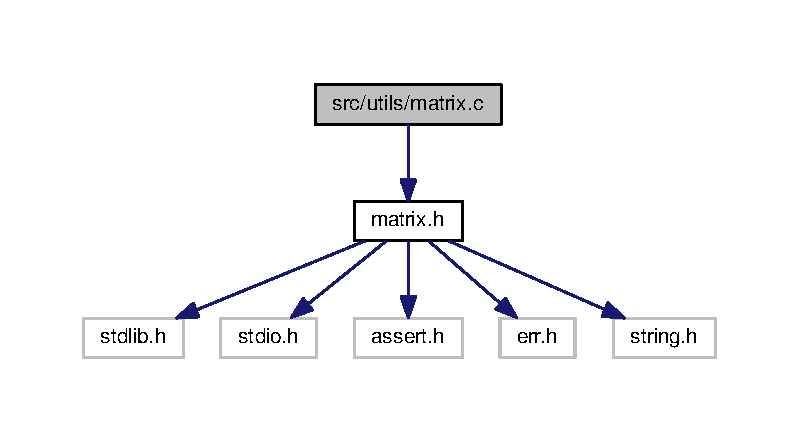
\includegraphics[width=350pt]{matrix_8c__incl}
\end{center}
\end{figure}
\subsection*{Functions}
\begin{DoxyCompactItemize}
\item 
struct \textbf{ matrix} $\ast$ \textbf{ matrix\+\_\+create} (size\+\_\+t rows, size\+\_\+t cols)
\item 
struct \textbf{ matrix} $\ast$ \textbf{ matrix\+\_\+create\+\_\+from\+\_\+array} (size\+\_\+t rows, size\+\_\+t cols, const double values[$\,$])
\item 
void \textbf{ matrix\+\_\+free} (struct \textbf{ matrix} $\ast$mx)
\item 
size\+\_\+t \textbf{ matrix\+\_\+rows} (const struct \textbf{ matrix} $\ast$mx)
\item 
size\+\_\+t \textbf{ matrix\+\_\+cols} (const struct \textbf{ matrix} $\ast$mx)
\item 
double \textbf{ matrix\+\_\+at} (const struct \textbf{ matrix} $\ast$mx, size\+\_\+t rows, size\+\_\+t cols)
\item 
void \textbf{ matrix\+\_\+set} (struct \textbf{ matrix} $\ast$mx, size\+\_\+t rows, size\+\_\+t cols, double value)
\item 
struct \textbf{ matrix} $\ast$ \textbf{ matrix\+\_\+copy} (const struct \textbf{ matrix} $\ast$mx)
\item 
void \textbf{ matrix\+\_\+transpose} (const struct \textbf{ matrix} $\ast$mx, struct \textbf{ matrix} $\ast$tmx)
\item 
void \textbf{ matrix\+\_\+sum} (const struct \textbf{ matrix} $\ast$mx1, const struct \textbf{ matrix} $\ast$mx2, struct \textbf{ matrix} $\ast$sum)
\item 
void \textbf{ matrix\+\_\+hadamard\+\_\+product} (const struct \textbf{ matrix} $\ast$mx1, const struct \textbf{ matrix} $\ast$mx2, struct \textbf{ matrix} $\ast$prod)
\item 
void \textbf{ matrix\+\_\+product} (const struct \textbf{ matrix} $\ast$mx1, const struct \textbf{ matrix} $\ast$mx2, struct \textbf{ matrix} $\ast$prod)
\item 
void \textbf{ matrix\+\_\+scale} (const struct \textbf{ matrix} $\ast$mx, double scale, struct \textbf{ matrix} $\ast$smx)
\item 
double \textbf{ matrix\+\_\+dot\+\_\+product} (const struct \textbf{ matrix} $\ast$v1, const struct \textbf{ matrix} $\ast$v2)
\item 
void \textbf{ matrix\+\_\+identity} (struct \textbf{ matrix} $\ast$mx)
\item 
int \textbf{ matrix\+\_\+is\+\_\+square} (const struct \textbf{ matrix} $\ast$mx)
\item 
int \textbf{ matrix\+\_\+is\+\_\+diagonal} (const struct \textbf{ matrix} $\ast$mx)
\item 
int \textbf{ matrix\+\_\+is\+\_\+upper\+\_\+triangulared} (const struct \textbf{ matrix} $\ast$mx)
\item 
void \textbf{ matrix\+\_\+diagonal} (const struct \textbf{ matrix} $\ast$v, struct \textbf{ matrix} $\ast$mx)
\item 
void \textbf{ matrix\+\_\+print} (const struct \textbf{ matrix} $\ast$mx)
\end{DoxyCompactItemize}


\subsection{Detailed Description}
Matrix implement. 

\begin{DoxyAuthor}{Author}
S4\+Master\+Race 
\end{DoxyAuthor}
\begin{DoxyVersion}{Version}
1.\+0 
\end{DoxyVersion}


\subsection{Function Documentation}
\mbox{\label{matrix_8c_ace105cd24473b52d67874132e81dd55b}} 
\index{matrix.\+c@{matrix.\+c}!matrix\+\_\+at@{matrix\+\_\+at}}
\index{matrix\+\_\+at@{matrix\+\_\+at}!matrix.\+c@{matrix.\+c}}
\subsubsection{matrix\+\_\+at()}
{\footnotesize\ttfamily double matrix\+\_\+at (\begin{DoxyParamCaption}\item[{const struct \textbf{ matrix} $\ast$}]{mx,  }\item[{size\+\_\+t}]{rows,  }\item[{size\+\_\+t}]{cols }\end{DoxyParamCaption})\hspace{0.3cm}{\ttfamily [inline]}}

Get value at {\ttfamily rows} rows and {\ttfamily cols} columns of {\ttfamily mx}


\begin{DoxyParams}{Parameters}
{\em mx} & a matrix \\
\hline
{\em rows} & rows \\
\hline
{\em cols} & columns \\
\hline
\end{DoxyParams}
\begin{DoxyReturn}{Returns}
the value at {\ttfamily rows} rows and {\ttfamily cols} columns of {\ttfamily mx}
\end{DoxyReturn}
\begin{DoxyPrecond}{Precondition}
{\ttfamily mx} must be not N\+U\+LL 

{\ttfamily rows} must be between {\ttfamily [0, matrix\+\_\+rows(mx)[} 

{\ttfamily cols} must be between {\ttfamily [0, matrix\+\_\+cols(mx)[}
\end{DoxyPrecond}
\begin{DoxyRemark}{Remarks}
Complexity\+: O(1) 
\end{DoxyRemark}
\mbox{\label{matrix_8c_a70ad38f54a8deaac09ddd554fa0ecccf}} 
\index{matrix.\+c@{matrix.\+c}!matrix\+\_\+cols@{matrix\+\_\+cols}}
\index{matrix\+\_\+cols@{matrix\+\_\+cols}!matrix.\+c@{matrix.\+c}}
\subsubsection{matrix\+\_\+cols()}
{\footnotesize\ttfamily size\+\_\+t matrix\+\_\+cols (\begin{DoxyParamCaption}\item[{const struct \textbf{ matrix} $\ast$}]{mx }\end{DoxyParamCaption})\hspace{0.3cm}{\ttfamily [inline]}}

Get the number of columns of {\ttfamily mx}


\begin{DoxyParams}{Parameters}
{\em mx} & a matrix \\
\hline
\end{DoxyParams}
\begin{DoxyReturn}{Returns}
the number of columns {\ttfamily mx}
\end{DoxyReturn}
\begin{DoxyPrecond}{Precondition}
{\ttfamily mx} must be not N\+U\+LL
\end{DoxyPrecond}
\begin{DoxyRemark}{Remarks}
Complexity\+: O(1) 
\end{DoxyRemark}
\mbox{\label{matrix_8c_a6663b065febb290385857b26fdb1a353}} 
\index{matrix.\+c@{matrix.\+c}!matrix\+\_\+copy@{matrix\+\_\+copy}}
\index{matrix\+\_\+copy@{matrix\+\_\+copy}!matrix.\+c@{matrix.\+c}}
\subsubsection{matrix\+\_\+copy()}
{\footnotesize\ttfamily struct \textbf{ matrix}$\ast$ matrix\+\_\+copy (\begin{DoxyParamCaption}\item[{const struct \textbf{ matrix} $\ast$}]{mx }\end{DoxyParamCaption})}

Copy the matrix {\ttfamily mx}


\begin{DoxyParams}{Parameters}
{\em mx} & a matrix \\
\hline
\end{DoxyParams}
\begin{DoxyReturn}{Returns}
the copy of {\ttfamily mx}
\end{DoxyReturn}
\begin{DoxyPrecond}{Precondition}
{\ttfamily mx} must be not N\+U\+LL
\end{DoxyPrecond}
\begin{DoxyRemark}{Remarks}
Complexity\+: O(1) 
\end{DoxyRemark}
\mbox{\label{matrix_8c_ad2d40d9c13eba774d6bb788021242a95}} 
\index{matrix.\+c@{matrix.\+c}!matrix\+\_\+create@{matrix\+\_\+create}}
\index{matrix\+\_\+create@{matrix\+\_\+create}!matrix.\+c@{matrix.\+c}}
\subsubsection{matrix\+\_\+create()}
{\footnotesize\ttfamily struct \textbf{ matrix}$\ast$ matrix\+\_\+create (\begin{DoxyParamCaption}\item[{size\+\_\+t}]{rows,  }\item[{size\+\_\+t}]{cols }\end{DoxyParamCaption})}

Create a matrix of size {\ttfamily rows} rows and {\ttfamily cols} columns


\begin{DoxyParams}{Parameters}
{\em rows} & number of rows \\
\hline
{\em cols} & number of columns\\
\hline
\end{DoxyParams}
\begin{DoxyReturn}{Returns}
the initialized matrix of size {\ttfamily rows} rows and {\ttfamily cols} columns
\end{DoxyReturn}
\begin{DoxyPrecond}{Precondition}
{\ttfamily rows} must be greater than zero 

{\ttfamily cols} must be greater than zero
\end{DoxyPrecond}
\begin{DoxyRemark}{Remarks}
Complexity\+: O(1) 
\end{DoxyRemark}
\mbox{\label{matrix_8c_a268a5429e2e4bc1664045624a82bc09c}} 
\index{matrix.\+c@{matrix.\+c}!matrix\+\_\+create\+\_\+from\+\_\+array@{matrix\+\_\+create\+\_\+from\+\_\+array}}
\index{matrix\+\_\+create\+\_\+from\+\_\+array@{matrix\+\_\+create\+\_\+from\+\_\+array}!matrix.\+c@{matrix.\+c}}
\subsubsection{matrix\+\_\+create\+\_\+from\+\_\+array()}
{\footnotesize\ttfamily struct \textbf{ matrix}$\ast$ matrix\+\_\+create\+\_\+from\+\_\+array (\begin{DoxyParamCaption}\item[{size\+\_\+t}]{rows,  }\item[{size\+\_\+t}]{cols,  }\item[{const double}]{values[$\,$] }\end{DoxyParamCaption})}

Create a matrix of size {\ttfamily rows} rows and {\ttfamily cols} columns from {\ttfamily values}


\begin{DoxyParams}{Parameters}
{\em rows} & number of rows \\
\hline
{\em cols} & number of columns \\
\hline
{\em values} & an array\\
\hline
\end{DoxyParams}
\begin{DoxyReturn}{Returns}
the initialized matrix of size {\ttfamily rows} rows and {\ttfamily cols} columns from {\ttfamily values}
\end{DoxyReturn}
\begin{DoxyPrecond}{Precondition}
{\ttfamily rows} must be greater than zero 

{\ttfamily cols} must be greater than zero 

{\ttfamily values} must be not N\+U\+LL
\end{DoxyPrecond}
\begin{DoxyRemark}{Remarks}
Complexity\+: O(\+N) 
\end{DoxyRemark}
\mbox{\label{matrix_8c_a74c9bd4f933938a77a0b30ef3204ab09}} 
\index{matrix.\+c@{matrix.\+c}!matrix\+\_\+diagonal@{matrix\+\_\+diagonal}}
\index{matrix\+\_\+diagonal@{matrix\+\_\+diagonal}!matrix.\+c@{matrix.\+c}}
\subsubsection{matrix\+\_\+diagonal()}
{\footnotesize\ttfamily void matrix\+\_\+diagonal (\begin{DoxyParamCaption}\item[{const struct \textbf{ matrix} $\ast$}]{v,  }\item[{struct \textbf{ matrix} $\ast$}]{mx }\end{DoxyParamCaption})}

Take a vector {\ttfamily v} and put it to the diagonal of {\ttfamily mx}


\begin{DoxyParams}{Parameters}
{\em v} & a vector \\
\hline
{\em mx} & a matrix\\
\hline
\end{DoxyParams}
\begin{DoxyPrecond}{Precondition}
{\ttfamily v} must be not N\+U\+LL 

{\ttfamily mx} must be not N\+U\+LL 

{\ttfamily matrix\+\_\+cols(v)} must be equal to one 

{\ttfamily matrix\+\_\+rows(v)} must be equel to {\ttfamily matrix\+\_\+rows(mx)} 

{\ttfamily matrix\+\_\+rows(mx)} must be equel to {\ttfamily matrix\+\_\+cols(mx)}
\end{DoxyPrecond}
\begin{DoxyPostcond}{Postcondition}
The diagonal of {\ttfamily mx} is {\ttfamily v} 
\end{DoxyPostcond}
\mbox{\label{matrix_8c_a7ba7365201acc5889936e1836d14cc8b}} 
\index{matrix.\+c@{matrix.\+c}!matrix\+\_\+dot\+\_\+product@{matrix\+\_\+dot\+\_\+product}}
\index{matrix\+\_\+dot\+\_\+product@{matrix\+\_\+dot\+\_\+product}!matrix.\+c@{matrix.\+c}}
\subsubsection{matrix\+\_\+dot\+\_\+product()}
{\footnotesize\ttfamily double matrix\+\_\+dot\+\_\+product (\begin{DoxyParamCaption}\item[{const struct \textbf{ matrix} $\ast$}]{v1,  }\item[{const struct \textbf{ matrix} $\ast$}]{v2 }\end{DoxyParamCaption})}

Do the dot product of vector {\ttfamily v1} with vector {\ttfamily v2}


\begin{DoxyParams}{Parameters}
{\em v1} & a vector \\
\hline
{\em v2} & a vector \\
\hline
\end{DoxyParams}
\begin{DoxyReturn}{Returns}
the dot product of vector {\ttfamily v1} with vector {\ttfamily v2}
\end{DoxyReturn}
\begin{DoxyPrecond}{Precondition}
{\ttfamily v1} must be not N\+U\+LL 

{\ttfamily v2} must be not N\+U\+LL 

{\ttfamily matrix\+\_\+cols(v1)} and {\ttfamily matrix\+\_\+cols(v2)} must be equal to one 

{\ttfamily matrix\+\_\+rows(v1)} must be equal to {\ttfamily matrix\+\_\+rows(v2)}
\end{DoxyPrecond}
\begin{DoxyRemark}{Remarks}
Complexity\+: O(\+N) 
\end{DoxyRemark}
\mbox{\label{matrix_8c_ac19cd61ef9f183a9b92d6789399f8646}} 
\index{matrix.\+c@{matrix.\+c}!matrix\+\_\+free@{matrix\+\_\+free}}
\index{matrix\+\_\+free@{matrix\+\_\+free}!matrix.\+c@{matrix.\+c}}
\subsubsection{matrix\+\_\+free()}
{\footnotesize\ttfamily void matrix\+\_\+free (\begin{DoxyParamCaption}\item[{struct \textbf{ matrix} $\ast$}]{mx }\end{DoxyParamCaption})\hspace{0.3cm}{\ttfamily [inline]}}

Free the matrix {\ttfamily mx}


\begin{DoxyParams}{Parameters}
{\em mx} & a matrix\\
\hline
\end{DoxyParams}
\begin{DoxyPrecond}{Precondition}
{\ttfamily mx} must be not N\+U\+LL
\end{DoxyPrecond}
\begin{DoxyPostcond}{Postcondition}
{\ttfamily mx} is freed
\end{DoxyPostcond}
\begin{DoxyRemark}{Remarks}
Complexity\+: O(1) 
\end{DoxyRemark}
\mbox{\label{matrix_8c_a52deb76b55ddbb957264866f5c856d0a}} 
\index{matrix.\+c@{matrix.\+c}!matrix\+\_\+hadamard\+\_\+product@{matrix\+\_\+hadamard\+\_\+product}}
\index{matrix\+\_\+hadamard\+\_\+product@{matrix\+\_\+hadamard\+\_\+product}!matrix.\+c@{matrix.\+c}}
\subsubsection{matrix\+\_\+hadamard\+\_\+product()}
{\footnotesize\ttfamily void matrix\+\_\+hadamard\+\_\+product (\begin{DoxyParamCaption}\item[{const struct \textbf{ matrix} $\ast$}]{mx1,  }\item[{const struct \textbf{ matrix} $\ast$}]{mx2,  }\item[{struct \textbf{ matrix} $\ast$}]{prod }\end{DoxyParamCaption})}

Do the hadamard product of matrix {\ttfamily mx1} with {\ttfamily mx2}


\begin{DoxyParams}{Parameters}
{\em mx1} & a matrix \\
\hline
{\em mx2} & a matrix \\
\hline
{\em prod} & a matrix\\
\hline
\end{DoxyParams}
\begin{DoxyPrecond}{Precondition}
{\ttfamily mx1} must be not N\+U\+LL 

{\ttfamily mx2} must be not N\+U\+LL 

{\ttfamily prod} must be not N\+U\+LL 

{\ttfamily matrix\+\_\+rows(mx1)} must be equal to {\ttfamily matrix\+\_\+rows(mx2)} 

{\ttfamily matrix\+\_\+cols(mx1)} must be equal to {\ttfamily matrix\+\_\+cols(mx2)} 

{\ttfamily matrix\+\_\+rows(prod)} must be equal to {\ttfamily matrix\+\_\+rows(mx1)} 

{\ttfamily matrix\+\_\+cols(prod)} must be equal to {\ttfamily matrix\+\_\+cols(mx1)}
\end{DoxyPrecond}
\begin{DoxyPostcond}{Postcondition}
{\ttfamily prod} is the hadamard product of matrix {\ttfamily mx1} with {\ttfamily mx2}
\end{DoxyPostcond}
\begin{DoxyRemark}{Remarks}
Complexity\+: O(\+N) 
\end{DoxyRemark}
\mbox{\label{matrix_8c_afa54c9d6ef22a1e0a0ca39221939b8c7}} 
\index{matrix.\+c@{matrix.\+c}!matrix\+\_\+identity@{matrix\+\_\+identity}}
\index{matrix\+\_\+identity@{matrix\+\_\+identity}!matrix.\+c@{matrix.\+c}}
\subsubsection{matrix\+\_\+identity()}
{\footnotesize\ttfamily void matrix\+\_\+identity (\begin{DoxyParamCaption}\item[{struct \textbf{ matrix} $\ast$}]{mx }\end{DoxyParamCaption})}

Set the matrix {\ttfamily mx} to an identity matrix


\begin{DoxyParams}{Parameters}
{\em mx} & a matrix\\
\hline
\end{DoxyParams}
\begin{DoxyPrecond}{Precondition}
{\ttfamily mx} must be not N\+U\+LL 

{\ttfamily matrix\+\_\+rows(mx)} must be equal to {\ttfamily matrix\+\_\+cols(mx)}
\end{DoxyPrecond}
\begin{DoxyPostcond}{Postcondition}
{\ttfamily mx} is an identity matrix
\end{DoxyPostcond}
\begin{DoxyRemark}{Remarks}
Complexity\+: O(\+N) 
\end{DoxyRemark}
\mbox{\label{matrix_8c_a2379a87492cbb3bf0c4fdc8e58589d1c}} 
\index{matrix.\+c@{matrix.\+c}!matrix\+\_\+is\+\_\+diagonal@{matrix\+\_\+is\+\_\+diagonal}}
\index{matrix\+\_\+is\+\_\+diagonal@{matrix\+\_\+is\+\_\+diagonal}!matrix.\+c@{matrix.\+c}}
\subsubsection{matrix\+\_\+is\+\_\+diagonal()}
{\footnotesize\ttfamily int matrix\+\_\+is\+\_\+diagonal (\begin{DoxyParamCaption}\item[{const struct \textbf{ matrix} $\ast$}]{mx }\end{DoxyParamCaption})\hspace{0.3cm}{\ttfamily [inline]}}

Check if the matrix {\ttfamily mx} is diagonaled


\begin{DoxyParams}{Parameters}
{\em mx} & a matrix \\
\hline
\end{DoxyParams}
\begin{DoxyReturn}{Returns}
{\ttfamily 1} if the matrix is diagonaled, {\ttfamily 0} otherwise
\end{DoxyReturn}
\begin{DoxyPrecond}{Precondition}
{\ttfamily mx} must be not N\+U\+LL
\end{DoxyPrecond}
\begin{DoxyRemark}{Remarks}
Complexity\+: O(\+N) 
\end{DoxyRemark}
\mbox{\label{matrix_8c_a0bc537e836547fd549f64464c938b1d2}} 
\index{matrix.\+c@{matrix.\+c}!matrix\+\_\+is\+\_\+square@{matrix\+\_\+is\+\_\+square}}
\index{matrix\+\_\+is\+\_\+square@{matrix\+\_\+is\+\_\+square}!matrix.\+c@{matrix.\+c}}
\subsubsection{matrix\+\_\+is\+\_\+square()}
{\footnotesize\ttfamily int matrix\+\_\+is\+\_\+square (\begin{DoxyParamCaption}\item[{const struct \textbf{ matrix} $\ast$}]{mx }\end{DoxyParamCaption})\hspace{0.3cm}{\ttfamily [inline]}}

Check if the matrix {\ttfamily mx} is squared


\begin{DoxyParams}{Parameters}
{\em mx} & a matrix \\
\hline
\end{DoxyParams}
\begin{DoxyReturn}{Returns}
{\ttfamily 1} if the matrix is squared, {\ttfamily 0} otherwise
\end{DoxyReturn}
\begin{DoxyPrecond}{Precondition}
{\ttfamily mx} must be not N\+U\+LL
\end{DoxyPrecond}
\begin{DoxyRemark}{Remarks}
Complexity\+: O(1) 
\end{DoxyRemark}
\mbox{\label{matrix_8c_ae3a4575aa2b0493bbf0b7bee70d30f07}} 
\index{matrix.\+c@{matrix.\+c}!matrix\+\_\+is\+\_\+upper\+\_\+triangulared@{matrix\+\_\+is\+\_\+upper\+\_\+triangulared}}
\index{matrix\+\_\+is\+\_\+upper\+\_\+triangulared@{matrix\+\_\+is\+\_\+upper\+\_\+triangulared}!matrix.\+c@{matrix.\+c}}
\subsubsection{matrix\+\_\+is\+\_\+upper\+\_\+triangulared()}
{\footnotesize\ttfamily int matrix\+\_\+is\+\_\+upper\+\_\+triangulared (\begin{DoxyParamCaption}\item[{const struct \textbf{ matrix} $\ast$}]{mx }\end{DoxyParamCaption})\hspace{0.3cm}{\ttfamily [inline]}}

Check if the matrix {\ttfamily mx} is upper triangulared


\begin{DoxyParams}{Parameters}
{\em mx} & a matrix \\
\hline
\end{DoxyParams}
\begin{DoxyReturn}{Returns}
{\ttfamily 1} if the matrix is upper triangulared, {\ttfamily 0} otherwise
\end{DoxyReturn}
\begin{DoxyPrecond}{Precondition}
{\ttfamily mx} must be not N\+U\+LL
\end{DoxyPrecond}
\begin{DoxyRemark}{Remarks}
Complexity\+: O(\+N) 
\end{DoxyRemark}
\mbox{\label{matrix_8c_a41f40f546c465fd096679a7f94ea5e8b}} 
\index{matrix.\+c@{matrix.\+c}!matrix\+\_\+print@{matrix\+\_\+print}}
\index{matrix\+\_\+print@{matrix\+\_\+print}!matrix.\+c@{matrix.\+c}}
\subsubsection{matrix\+\_\+print()}
{\footnotesize\ttfamily void matrix\+\_\+print (\begin{DoxyParamCaption}\item[{const struct \textbf{ matrix} $\ast$}]{mx }\end{DoxyParamCaption})}

Print the matrix {\ttfamily mx}


\begin{DoxyParams}{Parameters}
{\em mx} & a matrix\\
\hline
\end{DoxyParams}
\begin{DoxyPrecond}{Precondition}
{\ttfamily mx} must be not N\+U\+LL
\end{DoxyPrecond}
\begin{DoxyPostcond}{Postcondition}
Print the matrix {\ttfamily mx} 
\end{DoxyPostcond}
\mbox{\label{matrix_8c_a48e828fb00afc50e3616adefe87643bf}} 
\index{matrix.\+c@{matrix.\+c}!matrix\+\_\+product@{matrix\+\_\+product}}
\index{matrix\+\_\+product@{matrix\+\_\+product}!matrix.\+c@{matrix.\+c}}
\subsubsection{matrix\+\_\+product()}
{\footnotesize\ttfamily void matrix\+\_\+product (\begin{DoxyParamCaption}\item[{const struct \textbf{ matrix} $\ast$}]{mx1,  }\item[{const struct \textbf{ matrix} $\ast$}]{mx2,  }\item[{struct \textbf{ matrix} $\ast$}]{prod }\end{DoxyParamCaption})}

Multiply the matrix {\ttfamily mx1} with {\ttfamily mx2}


\begin{DoxyParams}{Parameters}
{\em mx1} & a matrix \\
\hline
{\em mx2} & a matrix \\
\hline
{\em prod} & a matrix\\
\hline
\end{DoxyParams}
\begin{DoxyPrecond}{Precondition}
{\ttfamily mx1} must be not N\+U\+LL 

{\ttfamily mx2} must be not N\+U\+LL 

{\ttfamily prod} must be not N\+U\+LL 

{\ttfamily prod} must be not equal to {\ttfamily mx1} 

{\ttfamily prod} must be not equal to {\ttfamily mx2} 

{\ttfamily matrix\+\_\+cols(mx1)} must be equal to {\ttfamily matrix\+\_\+rows(mx2)} 

{\ttfamily matrix\+\_\+rows(prod)} must be equal to {\ttfamily matrix\+\_\+rows(mx1)} 

{\ttfamily matrix\+\_\+cols(prod)} must be equal to {\ttfamily matrix\+\_\+cols(mx2)}
\end{DoxyPrecond}
\begin{DoxyPostcond}{Postcondition}
{\ttfamily prod} is the product of {\ttfamily mx1} with {\ttfamily mx2}
\end{DoxyPostcond}
\begin{DoxyRemark}{Remarks}
Complexity\+: O(nmp) 
\end{DoxyRemark}
\mbox{\label{matrix_8c_a7d9ca687a57f2328a02b9a056964b2fb}} 
\index{matrix.\+c@{matrix.\+c}!matrix\+\_\+rows@{matrix\+\_\+rows}}
\index{matrix\+\_\+rows@{matrix\+\_\+rows}!matrix.\+c@{matrix.\+c}}
\subsubsection{matrix\+\_\+rows()}
{\footnotesize\ttfamily size\+\_\+t matrix\+\_\+rows (\begin{DoxyParamCaption}\item[{const struct \textbf{ matrix} $\ast$}]{mx }\end{DoxyParamCaption})\hspace{0.3cm}{\ttfamily [inline]}}

Get the number of rows {\ttfamily mx}


\begin{DoxyParams}{Parameters}
{\em mx} & a matrix \\
\hline
\end{DoxyParams}
\begin{DoxyReturn}{Returns}
the number of rows of {\ttfamily mx}
\end{DoxyReturn}
\begin{DoxyPrecond}{Precondition}
{\ttfamily mx} must be not N\+U\+LL
\end{DoxyPrecond}
\begin{DoxyRemark}{Remarks}
Complexity\+: O(1) 
\end{DoxyRemark}
\mbox{\label{matrix_8c_aed3de5b6889de7358d66e2ac1b4c6efb}} 
\index{matrix.\+c@{matrix.\+c}!matrix\+\_\+scale@{matrix\+\_\+scale}}
\index{matrix\+\_\+scale@{matrix\+\_\+scale}!matrix.\+c@{matrix.\+c}}
\subsubsection{matrix\+\_\+scale()}
{\footnotesize\ttfamily void matrix\+\_\+scale (\begin{DoxyParamCaption}\item[{const struct \textbf{ matrix} $\ast$}]{mx,  }\item[{double}]{scale,  }\item[{struct \textbf{ matrix} $\ast$}]{smx }\end{DoxyParamCaption})}

Scale the matrix {\ttfamily mx} with {\ttfamily scale}


\begin{DoxyParams}{Parameters}
{\em mx} & a matrix \\
\hline
{\em scale} & the scale factor \\
\hline
{\em smx} & a matrix\\
\hline
\end{DoxyParams}
\begin{DoxyPrecond}{Precondition}
{\ttfamily mx} must be not N\+U\+LL 

{\ttfamily smx} must be not N\+U\+LL 

{\ttfamily matrix\+\_\+rows(smx)} must be equal to {\ttfamily matrix\+\_\+rows(mx)} 

{\ttfamily matrix\+\_\+cols(smx)} must be equal to {\ttfamily matrix\+\_\+cols(mx)}
\end{DoxyPrecond}
\begin{DoxyPostcond}{Postcondition}
{\ttfamily smx} is the {\ttfamily scale} scaled matrix of {\ttfamily mx}
\end{DoxyPostcond}
\begin{DoxyRemark}{Remarks}
Complexity\+: O(\+N) 
\end{DoxyRemark}
\mbox{\label{matrix_8c_a9e159c4c2c953106b7a1a4f0d4a03616}} 
\index{matrix.\+c@{matrix.\+c}!matrix\+\_\+set@{matrix\+\_\+set}}
\index{matrix\+\_\+set@{matrix\+\_\+set}!matrix.\+c@{matrix.\+c}}
\subsubsection{matrix\+\_\+set()}
{\footnotesize\ttfamily void matrix\+\_\+set (\begin{DoxyParamCaption}\item[{struct \textbf{ matrix} $\ast$}]{mx,  }\item[{size\+\_\+t}]{rows,  }\item[{size\+\_\+t}]{cols,  }\item[{double}]{value }\end{DoxyParamCaption})\hspace{0.3cm}{\ttfamily [inline]}}

Set the value at {\ttfamily rows} rows and {\ttfamily cols} columns with {\ttfamily value} of {\ttfamily mx}


\begin{DoxyParams}{Parameters}
{\em mx} & a matrix \\
\hline
{\em rows} & rows \\
\hline
{\em cols} & columns \\
\hline
{\em value} & a value\\
\hline
\end{DoxyParams}
\begin{DoxyPrecond}{Precondition}
{\ttfamily mx} must be not N\+U\+LL 

{\ttfamily rows} must be between {\ttfamily [0, matrix\+\_\+rows(mx)[} 

{\ttfamily cols} must be between {\ttfamily [0, matrix\+\_\+cols(mx)[}
\end{DoxyPrecond}
\begin{DoxyPostcond}{Postcondition}
the value at {\ttfamily rows} rows and {\ttfamily cols} columns is {\ttfamily value}
\end{DoxyPostcond}
\begin{DoxyRemark}{Remarks}
Complexity\+: O(1) 
\end{DoxyRemark}
\mbox{\label{matrix_8c_a4a7c4970506bd591d265596d41c7fa0f}} 
\index{matrix.\+c@{matrix.\+c}!matrix\+\_\+sum@{matrix\+\_\+sum}}
\index{matrix\+\_\+sum@{matrix\+\_\+sum}!matrix.\+c@{matrix.\+c}}
\subsubsection{matrix\+\_\+sum()}
{\footnotesize\ttfamily void matrix\+\_\+sum (\begin{DoxyParamCaption}\item[{const struct \textbf{ matrix} $\ast$}]{mx1,  }\item[{const struct \textbf{ matrix} $\ast$}]{mx2,  }\item[{struct \textbf{ matrix} $\ast$}]{sum }\end{DoxyParamCaption})}

Sum the matrix {\ttfamily mx1} with {\ttfamily mx2}


\begin{DoxyParams}{Parameters}
{\em mx1} & a matrix \\
\hline
{\em mx2} & a matrix \\
\hline
{\em sum} & a matrix\\
\hline
\end{DoxyParams}
\begin{DoxyPrecond}{Precondition}
{\ttfamily mx1} must be not N\+U\+LL 

{\ttfamily mx2} must be not N\+U\+LL 

{\ttfamily sum} must be not N\+U\+LL 

{\ttfamily matrix\+\_\+rows(mx1)} must be equal to {\ttfamily matrix\+\_\+rows(mx2)} 

{\ttfamily matrix\+\_\+cols(mx1)} must be equal to {\ttfamily matrix\+\_\+cols(mx2)} 

{\ttfamily matrix\+\_\+rows(sum)} must be equal to {\ttfamily matrix\+\_\+rows(mx1)} 

{\ttfamily matrix\+\_\+cols(sum)} must be equal to {\ttfamily matrix\+\_\+cols(mx1)}
\end{DoxyPrecond}
\begin{DoxyPostcond}{Postcondition}
{\ttfamily sum} is the sum of matrix {\ttfamily mx1} with {\ttfamily mx2}
\end{DoxyPostcond}
\begin{DoxyRemark}{Remarks}
Complexity\+: O(\+N) 
\end{DoxyRemark}
\mbox{\label{matrix_8c_ace9535ebf3fa66aa5aeed040eeccc1b3}} 
\index{matrix.\+c@{matrix.\+c}!matrix\+\_\+transpose@{matrix\+\_\+transpose}}
\index{matrix\+\_\+transpose@{matrix\+\_\+transpose}!matrix.\+c@{matrix.\+c}}
\subsubsection{matrix\+\_\+transpose()}
{\footnotesize\ttfamily void matrix\+\_\+transpose (\begin{DoxyParamCaption}\item[{const struct \textbf{ matrix} $\ast$}]{mx,  }\item[{struct \textbf{ matrix} $\ast$}]{tmx }\end{DoxyParamCaption})}

Transpose the matrix {\ttfamily mx}


\begin{DoxyParams}{Parameters}
{\em mx} & a matrix \\
\hline
{\em tmx} & a matrix\\
\hline
\end{DoxyParams}
\begin{DoxyPrecond}{Precondition}
{\ttfamily mx} must be not N\+U\+LL 

{\ttfamily tmx} must be not N\+U\+LL 

{\ttfamily tmx} must be not equal to {\ttfamily mx} 

{\ttfamily matrix\+\_\+rows(tmx)} must be equal to {\ttfamily matrix\+\_\+cols(mx)} 

{\ttfamily matrix\+\_\+cols(tmx)} must be equal to {\ttfamily matrix\+\_\+rows(mx)}
\end{DoxyPrecond}
\begin{DoxyPostcond}{Postcondition}
{\ttfamily tmx} is the transposed matrix of {\ttfamily mx}
\end{DoxyPostcond}
\begin{DoxyRemark}{Remarks}
Complexity\+: O(\+N) 
\end{DoxyRemark}

\section{src/utils/matrix.h File Reference}
\label{matrix_8h}\index{src/utils/matrix.\+h@{src/utils/matrix.\+h}}


Matrix implement.  


{\ttfamily \#include $<$stdlib.\+h$>$}\newline
{\ttfamily \#include $<$stdio.\+h$>$}\newline
{\ttfamily \#include $<$assert.\+h$>$}\newline
{\ttfamily \#include $<$err.\+h$>$}\newline
{\ttfamily \#include $<$string.\+h$>$}\newline
Include dependency graph for matrix.\+h\+:
\nopagebreak
\begin{figure}[H]
\begin{center}
\leavevmode
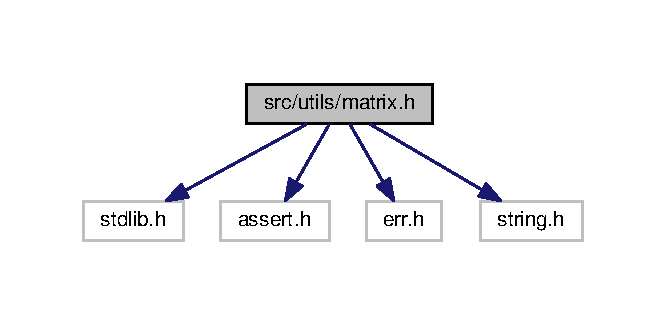
\includegraphics[width=350pt]{matrix_8h__incl}
\end{center}
\end{figure}
This graph shows which files directly or indirectly include this file\+:
\nopagebreak
\begin{figure}[H]
\begin{center}
\leavevmode
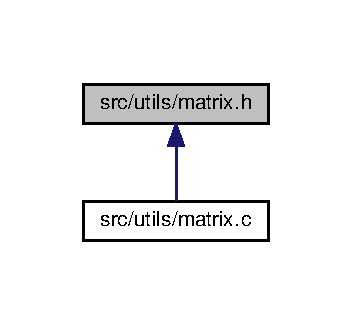
\includegraphics[width=169pt]{matrix_8h__dep__incl}
\end{center}
\end{figure}
\subsection*{Data Structures}
\begin{DoxyCompactItemize}
\item 
struct \textbf{ matrix}
\end{DoxyCompactItemize}
\subsection*{Functions}
\begin{DoxyCompactItemize}
\item 
struct \textbf{ matrix} $\ast$ \textbf{ matrix\+\_\+create} (size\+\_\+t rows, size\+\_\+t cols)
\item 
struct \textbf{ matrix} $\ast$ \textbf{ matrix\+\_\+create\+\_\+from\+\_\+array} (size\+\_\+t rows, size\+\_\+t cols, const double values[$\,$])
\item 
void \textbf{ matrix\+\_\+free} (struct \textbf{ matrix} $\ast$mx)
\item 
size\+\_\+t \textbf{ matrix\+\_\+rows} (const struct \textbf{ matrix} $\ast$mx)
\item 
size\+\_\+t \textbf{ matrix\+\_\+cols} (const struct \textbf{ matrix} $\ast$mx)
\item 
double \textbf{ matrix\+\_\+at} (const struct \textbf{ matrix} $\ast$mx, size\+\_\+t rows, size\+\_\+t cols)
\item 
void \textbf{ matrix\+\_\+set} (struct \textbf{ matrix} $\ast$mx, size\+\_\+t rows, size\+\_\+t cols, double value)
\item 
struct \textbf{ matrix} $\ast$ \textbf{ matrix\+\_\+copy} (const struct \textbf{ matrix} $\ast$mx)
\item 
void \textbf{ matrix\+\_\+transpose} (const struct \textbf{ matrix} $\ast$mx, struct \textbf{ matrix} $\ast$tmx)
\item 
void \textbf{ matrix\+\_\+sum} (const struct \textbf{ matrix} $\ast$mx1, const struct \textbf{ matrix} $\ast$mx2, struct \textbf{ matrix} $\ast$sum)
\item 
void \textbf{ matrix\+\_\+hadamard\+\_\+product} (const struct \textbf{ matrix} $\ast$mx1, const struct \textbf{ matrix} $\ast$mx2, struct \textbf{ matrix} $\ast$prod)
\item 
void \textbf{ matrix\+\_\+product} (const struct \textbf{ matrix} $\ast$mx1, const struct \textbf{ matrix} $\ast$mx2, struct \textbf{ matrix} $\ast$prod)
\item 
void \textbf{ matrix\+\_\+scale} (const struct \textbf{ matrix} $\ast$mx, double scale, struct \textbf{ matrix} $\ast$smx)
\item 
double \textbf{ matrix\+\_\+dot\+\_\+product} (const struct \textbf{ matrix} $\ast$v1, const struct \textbf{ matrix} $\ast$v2)
\item 
void \textbf{ matrix\+\_\+identity} (struct \textbf{ matrix} $\ast$mx)
\item 
int \textbf{ matrix\+\_\+is\+\_\+square} (const struct \textbf{ matrix} $\ast$mx)
\item 
int \textbf{ matrix\+\_\+is\+\_\+diagonal} (const struct \textbf{ matrix} $\ast$mx)
\item 
int \textbf{ matrix\+\_\+is\+\_\+upper\+\_\+triangulared} (const struct \textbf{ matrix} $\ast$mx)
\item 
void \textbf{ matrix\+\_\+diagonal} (const struct \textbf{ matrix} $\ast$v, struct \textbf{ matrix} $\ast$mx)
\item 
void \textbf{ matrix\+\_\+print} (const struct \textbf{ matrix} $\ast$mx)
\end{DoxyCompactItemize}


\subsection{Detailed Description}
Matrix implement. 

\begin{DoxyAuthor}{Author}
S4\+Master\+Race 
\end{DoxyAuthor}
\begin{DoxyVersion}{Version}
1.\+0 
\end{DoxyVersion}


\subsection{Function Documentation}
\mbox{\label{matrix_8h_ace105cd24473b52d67874132e81dd55b}} 
\index{matrix.\+h@{matrix.\+h}!matrix\+\_\+at@{matrix\+\_\+at}}
\index{matrix\+\_\+at@{matrix\+\_\+at}!matrix.\+h@{matrix.\+h}}
\subsubsection{matrix\+\_\+at()}
{\footnotesize\ttfamily double matrix\+\_\+at (\begin{DoxyParamCaption}\item[{const struct \textbf{ matrix} $\ast$}]{mx,  }\item[{size\+\_\+t}]{rows,  }\item[{size\+\_\+t}]{cols }\end{DoxyParamCaption})\hspace{0.3cm}{\ttfamily [inline]}}

Get value at {\ttfamily rows} rows and {\ttfamily cols} columns of {\ttfamily mx}


\begin{DoxyParams}{Parameters}
{\em mx} & a matrix \\
\hline
{\em rows} & rows \\
\hline
{\em cols} & columns \\
\hline
\end{DoxyParams}
\begin{DoxyReturn}{Returns}
the value at {\ttfamily rows} rows and {\ttfamily cols} columns of {\ttfamily mx}
\end{DoxyReturn}
\begin{DoxyPrecond}{Precondition}
{\ttfamily mx} must be not N\+U\+LL 

{\ttfamily rows} must be between {\ttfamily [0, matrix\+\_\+rows(mx)[} 

{\ttfamily cols} must be between {\ttfamily [0, matrix\+\_\+cols(mx)[}
\end{DoxyPrecond}
\begin{DoxyRemark}{Remarks}
Complexity\+: O(1) 
\end{DoxyRemark}
\mbox{\label{matrix_8h_a70ad38f54a8deaac09ddd554fa0ecccf}} 
\index{matrix.\+h@{matrix.\+h}!matrix\+\_\+cols@{matrix\+\_\+cols}}
\index{matrix\+\_\+cols@{matrix\+\_\+cols}!matrix.\+h@{matrix.\+h}}
\subsubsection{matrix\+\_\+cols()}
{\footnotesize\ttfamily size\+\_\+t matrix\+\_\+cols (\begin{DoxyParamCaption}\item[{const struct \textbf{ matrix} $\ast$}]{mx }\end{DoxyParamCaption})\hspace{0.3cm}{\ttfamily [inline]}}

Get the number of columns of {\ttfamily mx}


\begin{DoxyParams}{Parameters}
{\em mx} & a matrix \\
\hline
\end{DoxyParams}
\begin{DoxyReturn}{Returns}
the number of columns {\ttfamily mx}
\end{DoxyReturn}
\begin{DoxyPrecond}{Precondition}
{\ttfamily mx} must be not N\+U\+LL
\end{DoxyPrecond}
\begin{DoxyRemark}{Remarks}
Complexity\+: O(1) 
\end{DoxyRemark}
\mbox{\label{matrix_8h_a6663b065febb290385857b26fdb1a353}} 
\index{matrix.\+h@{matrix.\+h}!matrix\+\_\+copy@{matrix\+\_\+copy}}
\index{matrix\+\_\+copy@{matrix\+\_\+copy}!matrix.\+h@{matrix.\+h}}
\subsubsection{matrix\+\_\+copy()}
{\footnotesize\ttfamily struct \textbf{ matrix}$\ast$ matrix\+\_\+copy (\begin{DoxyParamCaption}\item[{const struct \textbf{ matrix} $\ast$}]{mx }\end{DoxyParamCaption})}

Copy the matrix {\ttfamily mx}


\begin{DoxyParams}{Parameters}
{\em mx} & a matrix \\
\hline
\end{DoxyParams}
\begin{DoxyReturn}{Returns}
the copy of {\ttfamily mx}
\end{DoxyReturn}
\begin{DoxyPrecond}{Precondition}
{\ttfamily mx} must be not N\+U\+LL
\end{DoxyPrecond}
\begin{DoxyRemark}{Remarks}
Complexity\+: O(1) 
\end{DoxyRemark}
\mbox{\label{matrix_8h_ad2d40d9c13eba774d6bb788021242a95}} 
\index{matrix.\+h@{matrix.\+h}!matrix\+\_\+create@{matrix\+\_\+create}}
\index{matrix\+\_\+create@{matrix\+\_\+create}!matrix.\+h@{matrix.\+h}}
\subsubsection{matrix\+\_\+create()}
{\footnotesize\ttfamily struct \textbf{ matrix}$\ast$ matrix\+\_\+create (\begin{DoxyParamCaption}\item[{size\+\_\+t}]{rows,  }\item[{size\+\_\+t}]{cols }\end{DoxyParamCaption})}

Create a matrix of size {\ttfamily rows} rows and {\ttfamily cols} columns


\begin{DoxyParams}{Parameters}
{\em rows} & number of rows \\
\hline
{\em cols} & number of columns\\
\hline
\end{DoxyParams}
\begin{DoxyReturn}{Returns}
the initialized matrix of size {\ttfamily rows} rows and {\ttfamily cols} columns
\end{DoxyReturn}
\begin{DoxyPrecond}{Precondition}
{\ttfamily rows} must be greater than zero 

{\ttfamily cols} must be greater than zero
\end{DoxyPrecond}
\begin{DoxyRemark}{Remarks}
Complexity\+: O(1) 
\end{DoxyRemark}
\mbox{\label{matrix_8h_a268a5429e2e4bc1664045624a82bc09c}} 
\index{matrix.\+h@{matrix.\+h}!matrix\+\_\+create\+\_\+from\+\_\+array@{matrix\+\_\+create\+\_\+from\+\_\+array}}
\index{matrix\+\_\+create\+\_\+from\+\_\+array@{matrix\+\_\+create\+\_\+from\+\_\+array}!matrix.\+h@{matrix.\+h}}
\subsubsection{matrix\+\_\+create\+\_\+from\+\_\+array()}
{\footnotesize\ttfamily struct \textbf{ matrix}$\ast$ matrix\+\_\+create\+\_\+from\+\_\+array (\begin{DoxyParamCaption}\item[{size\+\_\+t}]{rows,  }\item[{size\+\_\+t}]{cols,  }\item[{const double}]{values[$\,$] }\end{DoxyParamCaption})}

Create a matrix of size {\ttfamily rows} rows and {\ttfamily cols} columns from {\ttfamily values}


\begin{DoxyParams}{Parameters}
{\em rows} & number of rows \\
\hline
{\em cols} & number of columns \\
\hline
{\em values} & an array\\
\hline
\end{DoxyParams}
\begin{DoxyReturn}{Returns}
the initialized matrix of size {\ttfamily rows} rows and {\ttfamily cols} columns from {\ttfamily values}
\end{DoxyReturn}
\begin{DoxyPrecond}{Precondition}
{\ttfamily rows} must be greater than zero 

{\ttfamily cols} must be greater than zero 

{\ttfamily values} must be not N\+U\+LL
\end{DoxyPrecond}
\begin{DoxyRemark}{Remarks}
Complexity\+: O(\+N) 
\end{DoxyRemark}
\mbox{\label{matrix_8h_a74c9bd4f933938a77a0b30ef3204ab09}} 
\index{matrix.\+h@{matrix.\+h}!matrix\+\_\+diagonal@{matrix\+\_\+diagonal}}
\index{matrix\+\_\+diagonal@{matrix\+\_\+diagonal}!matrix.\+h@{matrix.\+h}}
\subsubsection{matrix\+\_\+diagonal()}
{\footnotesize\ttfamily void matrix\+\_\+diagonal (\begin{DoxyParamCaption}\item[{const struct \textbf{ matrix} $\ast$}]{v,  }\item[{struct \textbf{ matrix} $\ast$}]{mx }\end{DoxyParamCaption})}

Take a vector {\ttfamily v} and put it to the diagonal of {\ttfamily mx}


\begin{DoxyParams}{Parameters}
{\em v} & a vector \\
\hline
{\em mx} & a matrix\\
\hline
\end{DoxyParams}
\begin{DoxyPrecond}{Precondition}
{\ttfamily v} must be not N\+U\+LL 

{\ttfamily mx} must be not N\+U\+LL 

{\ttfamily matrix\+\_\+cols(v)} must be equal to one 

{\ttfamily matrix\+\_\+rows(v)} must be equel to {\ttfamily matrix\+\_\+rows(mx)} 

{\ttfamily matrix\+\_\+rows(mx)} must be equel to {\ttfamily matrix\+\_\+cols(mx)}
\end{DoxyPrecond}
\begin{DoxyPostcond}{Postcondition}
The diagonal of {\ttfamily mx} is {\ttfamily v} 
\end{DoxyPostcond}
\mbox{\label{matrix_8h_a7ba7365201acc5889936e1836d14cc8b}} 
\index{matrix.\+h@{matrix.\+h}!matrix\+\_\+dot\+\_\+product@{matrix\+\_\+dot\+\_\+product}}
\index{matrix\+\_\+dot\+\_\+product@{matrix\+\_\+dot\+\_\+product}!matrix.\+h@{matrix.\+h}}
\subsubsection{matrix\+\_\+dot\+\_\+product()}
{\footnotesize\ttfamily double matrix\+\_\+dot\+\_\+product (\begin{DoxyParamCaption}\item[{const struct \textbf{ matrix} $\ast$}]{v1,  }\item[{const struct \textbf{ matrix} $\ast$}]{v2 }\end{DoxyParamCaption})}

Do the dot product of vector {\ttfamily v1} with vector {\ttfamily v2}


\begin{DoxyParams}{Parameters}
{\em v1} & a vector \\
\hline
{\em v2} & a vector \\
\hline
\end{DoxyParams}
\begin{DoxyReturn}{Returns}
the dot product of vector {\ttfamily v1} with vector {\ttfamily v2}
\end{DoxyReturn}
\begin{DoxyPrecond}{Precondition}
{\ttfamily v1} must be not N\+U\+LL 

{\ttfamily v2} must be not N\+U\+LL 

{\ttfamily matrix\+\_\+cols(v1)} and {\ttfamily matrix\+\_\+cols(v2)} must be equal to one 

{\ttfamily matrix\+\_\+rows(v1)} must be equal to {\ttfamily matrix\+\_\+rows(v2)}
\end{DoxyPrecond}
\begin{DoxyRemark}{Remarks}
Complexity\+: O(\+N) 
\end{DoxyRemark}
\mbox{\label{matrix_8h_ac19cd61ef9f183a9b92d6789399f8646}} 
\index{matrix.\+h@{matrix.\+h}!matrix\+\_\+free@{matrix\+\_\+free}}
\index{matrix\+\_\+free@{matrix\+\_\+free}!matrix.\+h@{matrix.\+h}}
\subsubsection{matrix\+\_\+free()}
{\footnotesize\ttfamily void matrix\+\_\+free (\begin{DoxyParamCaption}\item[{struct \textbf{ matrix} $\ast$}]{mx }\end{DoxyParamCaption})\hspace{0.3cm}{\ttfamily [inline]}}

Free the matrix {\ttfamily mx}


\begin{DoxyParams}{Parameters}
{\em mx} & a matrix\\
\hline
\end{DoxyParams}
\begin{DoxyPrecond}{Precondition}
{\ttfamily mx} must be not N\+U\+LL
\end{DoxyPrecond}
\begin{DoxyPostcond}{Postcondition}
{\ttfamily mx} is freed
\end{DoxyPostcond}
\begin{DoxyRemark}{Remarks}
Complexity\+: O(1) 
\end{DoxyRemark}
\mbox{\label{matrix_8h_a52deb76b55ddbb957264866f5c856d0a}} 
\index{matrix.\+h@{matrix.\+h}!matrix\+\_\+hadamard\+\_\+product@{matrix\+\_\+hadamard\+\_\+product}}
\index{matrix\+\_\+hadamard\+\_\+product@{matrix\+\_\+hadamard\+\_\+product}!matrix.\+h@{matrix.\+h}}
\subsubsection{matrix\+\_\+hadamard\+\_\+product()}
{\footnotesize\ttfamily void matrix\+\_\+hadamard\+\_\+product (\begin{DoxyParamCaption}\item[{const struct \textbf{ matrix} $\ast$}]{mx1,  }\item[{const struct \textbf{ matrix} $\ast$}]{mx2,  }\item[{struct \textbf{ matrix} $\ast$}]{prod }\end{DoxyParamCaption})}

Do the hadamard product of matrix {\ttfamily mx1} with {\ttfamily mx2}


\begin{DoxyParams}{Parameters}
{\em mx1} & a matrix \\
\hline
{\em mx2} & a matrix \\
\hline
{\em prod} & a matrix\\
\hline
\end{DoxyParams}
\begin{DoxyPrecond}{Precondition}
{\ttfamily mx1} must be not N\+U\+LL 

{\ttfamily mx2} must be not N\+U\+LL 

{\ttfamily prod} must be not N\+U\+LL 

{\ttfamily matrix\+\_\+rows(mx1)} must be equal to {\ttfamily matrix\+\_\+rows(mx2)} 

{\ttfamily matrix\+\_\+cols(mx1)} must be equal to {\ttfamily matrix\+\_\+cols(mx2)} 

{\ttfamily matrix\+\_\+rows(prod)} must be equal to {\ttfamily matrix\+\_\+rows(mx1)} 

{\ttfamily matrix\+\_\+cols(prod)} must be equal to {\ttfamily matrix\+\_\+cols(mx1)}
\end{DoxyPrecond}
\begin{DoxyPostcond}{Postcondition}
{\ttfamily prod} is the hadamard product of matrix {\ttfamily mx1} with {\ttfamily mx2}
\end{DoxyPostcond}
\begin{DoxyRemark}{Remarks}
Complexity\+: O(\+N) 
\end{DoxyRemark}
\mbox{\label{matrix_8h_afa54c9d6ef22a1e0a0ca39221939b8c7}} 
\index{matrix.\+h@{matrix.\+h}!matrix\+\_\+identity@{matrix\+\_\+identity}}
\index{matrix\+\_\+identity@{matrix\+\_\+identity}!matrix.\+h@{matrix.\+h}}
\subsubsection{matrix\+\_\+identity()}
{\footnotesize\ttfamily void matrix\+\_\+identity (\begin{DoxyParamCaption}\item[{struct \textbf{ matrix} $\ast$}]{mx }\end{DoxyParamCaption})}

Set the matrix {\ttfamily mx} to an identity matrix


\begin{DoxyParams}{Parameters}
{\em mx} & a matrix\\
\hline
\end{DoxyParams}
\begin{DoxyPrecond}{Precondition}
{\ttfamily mx} must be not N\+U\+LL 

{\ttfamily matrix\+\_\+rows(mx)} must be equal to {\ttfamily matrix\+\_\+cols(mx)}
\end{DoxyPrecond}
\begin{DoxyPostcond}{Postcondition}
{\ttfamily mx} is an identity matrix
\end{DoxyPostcond}
\begin{DoxyRemark}{Remarks}
Complexity\+: O(\+N) 
\end{DoxyRemark}
\mbox{\label{matrix_8h_a2379a87492cbb3bf0c4fdc8e58589d1c}} 
\index{matrix.\+h@{matrix.\+h}!matrix\+\_\+is\+\_\+diagonal@{matrix\+\_\+is\+\_\+diagonal}}
\index{matrix\+\_\+is\+\_\+diagonal@{matrix\+\_\+is\+\_\+diagonal}!matrix.\+h@{matrix.\+h}}
\subsubsection{matrix\+\_\+is\+\_\+diagonal()}
{\footnotesize\ttfamily int matrix\+\_\+is\+\_\+diagonal (\begin{DoxyParamCaption}\item[{const struct \textbf{ matrix} $\ast$}]{mx }\end{DoxyParamCaption})\hspace{0.3cm}{\ttfamily [inline]}}

Check if the matrix {\ttfamily mx} is diagonaled


\begin{DoxyParams}{Parameters}
{\em mx} & a matrix \\
\hline
\end{DoxyParams}
\begin{DoxyReturn}{Returns}
{\ttfamily 1} if the matrix is diagonaled, {\ttfamily 0} otherwise
\end{DoxyReturn}
\begin{DoxyPrecond}{Precondition}
{\ttfamily mx} must be not N\+U\+LL
\end{DoxyPrecond}
\begin{DoxyRemark}{Remarks}
Complexity\+: O(\+N) 
\end{DoxyRemark}
\mbox{\label{matrix_8h_a0bc537e836547fd549f64464c938b1d2}} 
\index{matrix.\+h@{matrix.\+h}!matrix\+\_\+is\+\_\+square@{matrix\+\_\+is\+\_\+square}}
\index{matrix\+\_\+is\+\_\+square@{matrix\+\_\+is\+\_\+square}!matrix.\+h@{matrix.\+h}}
\subsubsection{matrix\+\_\+is\+\_\+square()}
{\footnotesize\ttfamily int matrix\+\_\+is\+\_\+square (\begin{DoxyParamCaption}\item[{const struct \textbf{ matrix} $\ast$}]{mx }\end{DoxyParamCaption})\hspace{0.3cm}{\ttfamily [inline]}}

Check if the matrix {\ttfamily mx} is squared


\begin{DoxyParams}{Parameters}
{\em mx} & a matrix \\
\hline
\end{DoxyParams}
\begin{DoxyReturn}{Returns}
{\ttfamily 1} if the matrix is squared, {\ttfamily 0} otherwise
\end{DoxyReturn}
\begin{DoxyPrecond}{Precondition}
{\ttfamily mx} must be not N\+U\+LL
\end{DoxyPrecond}
\begin{DoxyRemark}{Remarks}
Complexity\+: O(1) 
\end{DoxyRemark}
\mbox{\label{matrix_8h_ae3a4575aa2b0493bbf0b7bee70d30f07}} 
\index{matrix.\+h@{matrix.\+h}!matrix\+\_\+is\+\_\+upper\+\_\+triangulared@{matrix\+\_\+is\+\_\+upper\+\_\+triangulared}}
\index{matrix\+\_\+is\+\_\+upper\+\_\+triangulared@{matrix\+\_\+is\+\_\+upper\+\_\+triangulared}!matrix.\+h@{matrix.\+h}}
\subsubsection{matrix\+\_\+is\+\_\+upper\+\_\+triangulared()}
{\footnotesize\ttfamily int matrix\+\_\+is\+\_\+upper\+\_\+triangulared (\begin{DoxyParamCaption}\item[{const struct \textbf{ matrix} $\ast$}]{mx }\end{DoxyParamCaption})\hspace{0.3cm}{\ttfamily [inline]}}

Check if the matrix {\ttfamily mx} is upper triangulared


\begin{DoxyParams}{Parameters}
{\em mx} & a matrix \\
\hline
\end{DoxyParams}
\begin{DoxyReturn}{Returns}
{\ttfamily 1} if the matrix is upper triangulared, {\ttfamily 0} otherwise
\end{DoxyReturn}
\begin{DoxyPrecond}{Precondition}
{\ttfamily mx} must be not N\+U\+LL
\end{DoxyPrecond}
\begin{DoxyRemark}{Remarks}
Complexity\+: O(\+N) 
\end{DoxyRemark}
\mbox{\label{matrix_8h_a41f40f546c465fd096679a7f94ea5e8b}} 
\index{matrix.\+h@{matrix.\+h}!matrix\+\_\+print@{matrix\+\_\+print}}
\index{matrix\+\_\+print@{matrix\+\_\+print}!matrix.\+h@{matrix.\+h}}
\subsubsection{matrix\+\_\+print()}
{\footnotesize\ttfamily void matrix\+\_\+print (\begin{DoxyParamCaption}\item[{const struct \textbf{ matrix} $\ast$}]{mx }\end{DoxyParamCaption})}

Print the matrix {\ttfamily mx}


\begin{DoxyParams}{Parameters}
{\em mx} & a matrix\\
\hline
\end{DoxyParams}
\begin{DoxyPrecond}{Precondition}
{\ttfamily mx} must be not N\+U\+LL
\end{DoxyPrecond}
\begin{DoxyPostcond}{Postcondition}
Print the matrix {\ttfamily mx} 
\end{DoxyPostcond}
\mbox{\label{matrix_8h_a48e828fb00afc50e3616adefe87643bf}} 
\index{matrix.\+h@{matrix.\+h}!matrix\+\_\+product@{matrix\+\_\+product}}
\index{matrix\+\_\+product@{matrix\+\_\+product}!matrix.\+h@{matrix.\+h}}
\subsubsection{matrix\+\_\+product()}
{\footnotesize\ttfamily void matrix\+\_\+product (\begin{DoxyParamCaption}\item[{const struct \textbf{ matrix} $\ast$}]{mx1,  }\item[{const struct \textbf{ matrix} $\ast$}]{mx2,  }\item[{struct \textbf{ matrix} $\ast$}]{prod }\end{DoxyParamCaption})}

Multiply the matrix {\ttfamily mx1} with {\ttfamily mx2}


\begin{DoxyParams}{Parameters}
{\em mx1} & a matrix \\
\hline
{\em mx2} & a matrix \\
\hline
{\em prod} & a matrix\\
\hline
\end{DoxyParams}
\begin{DoxyPrecond}{Precondition}
{\ttfamily mx1} must be not N\+U\+LL 

{\ttfamily mx2} must be not N\+U\+LL 

{\ttfamily prod} must be not N\+U\+LL 

{\ttfamily prod} must be not equal to {\ttfamily mx1} 

{\ttfamily prod} must be not equal to {\ttfamily mx2} 

{\ttfamily matrix\+\_\+cols(mx1)} must be equal to {\ttfamily matrix\+\_\+rows(mx2)} 

{\ttfamily matrix\+\_\+rows(prod)} must be equal to {\ttfamily matrix\+\_\+rows(mx1)} 

{\ttfamily matrix\+\_\+cols(prod)} must be equal to {\ttfamily matrix\+\_\+cols(mx2)}
\end{DoxyPrecond}
\begin{DoxyPostcond}{Postcondition}
{\ttfamily prod} is the product of {\ttfamily mx1} with {\ttfamily mx2}
\end{DoxyPostcond}
\begin{DoxyRemark}{Remarks}
Complexity\+: O(nmp) 
\end{DoxyRemark}
\mbox{\label{matrix_8h_a7d9ca687a57f2328a02b9a056964b2fb}} 
\index{matrix.\+h@{matrix.\+h}!matrix\+\_\+rows@{matrix\+\_\+rows}}
\index{matrix\+\_\+rows@{matrix\+\_\+rows}!matrix.\+h@{matrix.\+h}}
\subsubsection{matrix\+\_\+rows()}
{\footnotesize\ttfamily size\+\_\+t matrix\+\_\+rows (\begin{DoxyParamCaption}\item[{const struct \textbf{ matrix} $\ast$}]{mx }\end{DoxyParamCaption})\hspace{0.3cm}{\ttfamily [inline]}}

Get the number of rows {\ttfamily mx}


\begin{DoxyParams}{Parameters}
{\em mx} & a matrix \\
\hline
\end{DoxyParams}
\begin{DoxyReturn}{Returns}
the number of rows of {\ttfamily mx}
\end{DoxyReturn}
\begin{DoxyPrecond}{Precondition}
{\ttfamily mx} must be not N\+U\+LL
\end{DoxyPrecond}
\begin{DoxyRemark}{Remarks}
Complexity\+: O(1) 
\end{DoxyRemark}
\mbox{\label{matrix_8h_aed3de5b6889de7358d66e2ac1b4c6efb}} 
\index{matrix.\+h@{matrix.\+h}!matrix\+\_\+scale@{matrix\+\_\+scale}}
\index{matrix\+\_\+scale@{matrix\+\_\+scale}!matrix.\+h@{matrix.\+h}}
\subsubsection{matrix\+\_\+scale()}
{\footnotesize\ttfamily void matrix\+\_\+scale (\begin{DoxyParamCaption}\item[{const struct \textbf{ matrix} $\ast$}]{mx,  }\item[{double}]{scale,  }\item[{struct \textbf{ matrix} $\ast$}]{smx }\end{DoxyParamCaption})}

Scale the matrix {\ttfamily mx} with {\ttfamily scale}


\begin{DoxyParams}{Parameters}
{\em mx} & a matrix \\
\hline
{\em scale} & the scale factor \\
\hline
{\em smx} & a matrix\\
\hline
\end{DoxyParams}
\begin{DoxyPrecond}{Precondition}
{\ttfamily mx} must be not N\+U\+LL 

{\ttfamily smx} must be not N\+U\+LL 

{\ttfamily matrix\+\_\+rows(smx)} must be equal to {\ttfamily matrix\+\_\+rows(mx)} 

{\ttfamily matrix\+\_\+cols(smx)} must be equal to {\ttfamily matrix\+\_\+cols(mx)}
\end{DoxyPrecond}
\begin{DoxyPostcond}{Postcondition}
{\ttfamily smx} is the {\ttfamily scale} scaled matrix of {\ttfamily mx}
\end{DoxyPostcond}
\begin{DoxyRemark}{Remarks}
Complexity\+: O(\+N) 
\end{DoxyRemark}
\mbox{\label{matrix_8h_a9e159c4c2c953106b7a1a4f0d4a03616}} 
\index{matrix.\+h@{matrix.\+h}!matrix\+\_\+set@{matrix\+\_\+set}}
\index{matrix\+\_\+set@{matrix\+\_\+set}!matrix.\+h@{matrix.\+h}}
\subsubsection{matrix\+\_\+set()}
{\footnotesize\ttfamily void matrix\+\_\+set (\begin{DoxyParamCaption}\item[{struct \textbf{ matrix} $\ast$}]{mx,  }\item[{size\+\_\+t}]{rows,  }\item[{size\+\_\+t}]{cols,  }\item[{double}]{value }\end{DoxyParamCaption})\hspace{0.3cm}{\ttfamily [inline]}}

Set the value at {\ttfamily rows} rows and {\ttfamily cols} columns with {\ttfamily value} of {\ttfamily mx}


\begin{DoxyParams}{Parameters}
{\em mx} & a matrix \\
\hline
{\em rows} & rows \\
\hline
{\em cols} & columns \\
\hline
{\em value} & a value\\
\hline
\end{DoxyParams}
\begin{DoxyPrecond}{Precondition}
{\ttfamily mx} must be not N\+U\+LL 

{\ttfamily rows} must be between {\ttfamily [0, matrix\+\_\+rows(mx)[} 

{\ttfamily cols} must be between {\ttfamily [0, matrix\+\_\+cols(mx)[}
\end{DoxyPrecond}
\begin{DoxyPostcond}{Postcondition}
the value at {\ttfamily rows} rows and {\ttfamily cols} columns is {\ttfamily value}
\end{DoxyPostcond}
\begin{DoxyRemark}{Remarks}
Complexity\+: O(1) 
\end{DoxyRemark}
\mbox{\label{matrix_8h_a4a7c4970506bd591d265596d41c7fa0f}} 
\index{matrix.\+h@{matrix.\+h}!matrix\+\_\+sum@{matrix\+\_\+sum}}
\index{matrix\+\_\+sum@{matrix\+\_\+sum}!matrix.\+h@{matrix.\+h}}
\subsubsection{matrix\+\_\+sum()}
{\footnotesize\ttfamily void matrix\+\_\+sum (\begin{DoxyParamCaption}\item[{const struct \textbf{ matrix} $\ast$}]{mx1,  }\item[{const struct \textbf{ matrix} $\ast$}]{mx2,  }\item[{struct \textbf{ matrix} $\ast$}]{sum }\end{DoxyParamCaption})}

Sum the matrix {\ttfamily mx1} with {\ttfamily mx2}


\begin{DoxyParams}{Parameters}
{\em mx1} & a matrix \\
\hline
{\em mx2} & a matrix \\
\hline
{\em sum} & a matrix\\
\hline
\end{DoxyParams}
\begin{DoxyPrecond}{Precondition}
{\ttfamily mx1} must be not N\+U\+LL 

{\ttfamily mx2} must be not N\+U\+LL 

{\ttfamily sum} must be not N\+U\+LL 

{\ttfamily matrix\+\_\+rows(mx1)} must be equal to {\ttfamily matrix\+\_\+rows(mx2)} 

{\ttfamily matrix\+\_\+cols(mx1)} must be equal to {\ttfamily matrix\+\_\+cols(mx2)} 

{\ttfamily matrix\+\_\+rows(sum)} must be equal to {\ttfamily matrix\+\_\+rows(mx1)} 

{\ttfamily matrix\+\_\+cols(sum)} must be equal to {\ttfamily matrix\+\_\+cols(mx1)}
\end{DoxyPrecond}
\begin{DoxyPostcond}{Postcondition}
{\ttfamily sum} is the sum of matrix {\ttfamily mx1} with {\ttfamily mx2}
\end{DoxyPostcond}
\begin{DoxyRemark}{Remarks}
Complexity\+: O(\+N) 
\end{DoxyRemark}
\mbox{\label{matrix_8h_ace9535ebf3fa66aa5aeed040eeccc1b3}} 
\index{matrix.\+h@{matrix.\+h}!matrix\+\_\+transpose@{matrix\+\_\+transpose}}
\index{matrix\+\_\+transpose@{matrix\+\_\+transpose}!matrix.\+h@{matrix.\+h}}
\subsubsection{matrix\+\_\+transpose()}
{\footnotesize\ttfamily void matrix\+\_\+transpose (\begin{DoxyParamCaption}\item[{const struct \textbf{ matrix} $\ast$}]{mx,  }\item[{struct \textbf{ matrix} $\ast$}]{tmx }\end{DoxyParamCaption})}

Transpose the matrix {\ttfamily mx}


\begin{DoxyParams}{Parameters}
{\em mx} & a matrix \\
\hline
{\em tmx} & a matrix\\
\hline
\end{DoxyParams}
\begin{DoxyPrecond}{Precondition}
{\ttfamily mx} must be not N\+U\+LL 

{\ttfamily tmx} must be not N\+U\+LL 

{\ttfamily tmx} must be not equal to {\ttfamily mx} 

{\ttfamily matrix\+\_\+rows(tmx)} must be equal to {\ttfamily matrix\+\_\+cols(mx)} 

{\ttfamily matrix\+\_\+cols(tmx)} must be equal to {\ttfamily matrix\+\_\+rows(mx)}
\end{DoxyPrecond}
\begin{DoxyPostcond}{Postcondition}
{\ttfamily tmx} is the transposed matrix of {\ttfamily mx}
\end{DoxyPostcond}
\begin{DoxyRemark}{Remarks}
Complexity\+: O(\+N) 
\end{DoxyRemark}

%--- End generated contents ---

% Index
\backmatter
\newpage
\phantomsection
\clearemptydoublepage
\addcontentsline{toc}{chapter}{Index}
\printindex

\end{document}
